% Note that the a4paper option is mainly intended so that authors in
% countries using A4 can easily print to A4 and see how their papers will
% look in print - the typesetting of the document will not typically be
% affected with changes in paper size (but the bottom and side margins will).
% Use the testflow package mentioned above to verify correct handling of
% both paper sizes by the user's LaTeX system.
%
% Also note that the "draftcls" or "draftclsnofoot", not "draft", option
% should be used if it is desired that the figures are to be displayed in
% draft mode.
%
\documentclass[a4paper,12pt]{report}

\linespread{1.5} \setlength{\parskip}{0.3cm}
% Add the compsoc option for Computer Society conferences.
%
% If IEEEtran.cls has not been installed into the LaTeX system files,
% manually specify the path to it like:
% \documentclass[conference]{../sty/IEEEtran}


\usepackage{amssymb}
\usepackage{amsmath}
\usepackage{amsthm}
\usepackage{latexsym}
\usepackage{algorithm}
\usepackage{algpseudocode}
\usepackage{graphicx} 
\usepackage{tabularx,array}
\usepackage{amsfonts}
\usepackage{amsmath}
\usepackage{epsfig}
\usepackage{verbatim}
%\usepackage{subfigure}
\usepackage{wallpaper}
\CenterWallPaper{.35}{ccu}


% Some very useful LaTeX packages include:
% (uncomment the ones you want to load)


% *** MISC UTILITY PACKAGES ***
%
%\usepackage{ifpdf}
% Heiko Oberdiek's ifpdf.sty is very useful if you need conditional
% compilation based on whether the output is pdf or dvi.
% usage:
% \ifpdf
%   % pdf code
% \else
%   % dvi code
% \fi
% The latest version of ifpdf.sty can be obtained from:
% http://www.ctan.org/tex-archive/macros/latex/contrib/oberdiek/
% Also, note that IEEEtran.cls V1.7 and later provides a builtin
% \ifCLASSINFOpdf conditional that works the same way.
% When switching from latex to pdflatex and vice-versa, the compiler may
% have to be run twice to clear warning/error messages.


% *** CITATION PACKAGES ***
%
\usepackage{cite}
% cite.sty was written by Donald Arseneau
% V1.6 and later of IEEEtran pre-defines the format of the cite.sty package
% \cite{} output to follow that of IEEE. Loading the cite package will
% result in citation numbers being automatically sorted and properly
% "compressed/ranged". e.g., [1], [9], [2], [7], [5], [6] without using
% cite.sty will become [1], [2], [5]--[7], [9] using cite.sty. cite.sty's
% \cite will automatically add leading space, if needed. Use cite.sty's
% noadjust option (cite.sty V3.8 and later) if you want to turn this off.
% cite.sty is already installed on most LaTeX systems. Be sure and use
% version 4.0 (2003-05-27) and later if using hyperref.sty. cite.sty does
% not currently provide for hyperlinked citations.
% The latest version can be obtained at:
% http://www.ctan.org/tex-archive/macros/latex/contrib/cite/
% The documentation is contained in the cite.sty file itself.
\usepackage{amsmath}
\usepackage{longtable}
\newcommand{\tabincell}[2]{\begin{tabular}{@{}#1@{}}#2\end{tabular}}%放在导言区 



% *** GRAPHICS RELATED PACKAGES ***
%
%\ifCLASSINFOpdf
 %  \usepackage[pdftex]{graphicx}
  % declare the path(s) where your graphic files are
  % \graphicspath{{../pdf/}{../jpeg/}}
  % and their extensions so you won't have to specify these with
  % every instance of \includegraphics
  % \DeclareGraphicsExtensions{.pdf,.jpeg,.png}
%\else
  % or other class option (dvipsone, dvipdf, if not using dvips). graphicx
  % will default to the driver specified in the system graphics.cfg if no
  % driver is specified.
 %  \usepackage[dvips]{graphicx}
  % declare the path(s) where your graphic files are
  % \graphicspath{{../eps/}}
  % and their extensions so you won't have to specify these with
  % every instance of \includegraphics
  % \DeclareGraphicsExtensions{.eps}
%\fi
% graphicx was written by David Carlisle and Sebastian Rahtz. It is
% required if you want graphics, photos, etc. graphicx.sty is already
% installed on most LaTeX systems. The latest version and documentation can
% be obtained at:
% http://www.ctan.org/tex-archive/macros/latex/required/graphics/
% Another good source of documentation is "Using Imported Graphics in
% LaTeX2e" by Keith Reckdahl which can be found as epslatex.ps or
% epslatex.pdf at: http://www.ctan.org/tex-archive/info/
%
% latex, and pdflatex in dvi mode, support graphics in encapsulated
% postscript (.eps) format. pdflatex in pdf mode supports graphics
% in .pdf, .jpeg, .png and .mps (metapost) formats. Users should ensure
% that all non-photo figures use a vector format (.eps, .pdf, .mps) and
% not a bitmapped formats (.jpeg, .png). IEEE frowns on bitmapped formats
% which can result in "jaggedy"/blurry rendering of lines and letters as
% well as large increases in file sizes.
%
% You can find documentation about the pdfTeX application at:
% http://www.tug.org/applications/pdftex



\usepackage{float}

% *** MATH PACKAGES ***
%
%\usepackage[cmex10]{amsmath}
% A popular package from the American Mathematical Society that provides
% many useful and powerful commands for dealing with mathematics. If using
% it, be sure to load this package with the cmex10 option to ensure that
% only type 1 fonts will utilized at all point sizes. Without this option,
% it is possible that some math symbols, particularly those within
% footnotes, will be rendered in bitmap form which will result in a
% document that can not be IEEE Xplore compliant!
%
% Also, note that the amsmath package sets \interdisplaylinepenalty to 10000
% thus preventing page breaks from occurring within multiline equations. Use:
%\interdisplaylinepenalty=2500
% after loading amsmath to restore such page breaks as IEEEtran.cls normally
% does. amsmath.sty is already installed on most LaTeX systems. The latest
% version and documentation can be obtained at:
% http://www.ctan.org/tex-archive/macros/latex/required/amslatex/math/





% *** SPECIALIZED LIST PACKAGES ***
%
%\usepackage{algorithmic}
% algorithmic.sty was written by Peter Williams and Rogerio Brito.
% This package provides an algorithmic environment fo describing algorithms.
% You can use the algorithmic environment in-text or within a figure
% environment to provide for a floating algorithm. Do NOT use the algorithm
% floating environment provided by algorithm.sty (by the same authors) or
% algorithm2e.sty (by Christophe Fiorio) as IEEE does not use dedicated
% algorithm float types and packages that provide these will not provide
% correct IEEE style captions. The latest version and documentation of
% algorithmic.sty can be obtained at:
% http://www.ctan.org/tex-archive/macros/latex/contrib/algorithms/
% There is also a support site at:
% http://algorithms.berlios.de/index.html
% Also of interest may be the (relatively newer and more customizable)
% algorithmicx.sty package by Szasz Janos:
% http://www.ctan.org/tex-archive/macros/latex/contrib/algorithmicx/




% *** ALIGNMENT PACKAGES ***
%
%\usepackage{array}
% Frank Mittelbach's and David Carlisle's array.sty patches and improves
% the standard LaTeX2e array and tabular environments to provide better
% appearance and additional user controls. As the default LaTeX2e table
% generation code is lacking to the point of almost being broken with
% respect to the quality of the end results, all users are strongly
% advised to use an enhanced (at the very least that provided by array.sty)
% set of table tools. array.sty is already installed on most systems. The
% latest version and documentation can be obtained at:
% http://www.ctan.org/tex-archive/macros/latex/required/tools/


%\usepackage{mdwmath}
%\usepackage{mdwtab}
% Also highly recommended is Mark Wooding's extremely powerful MDW tools,
% especially mdwmath.sty and mdwtab.sty which are used to format equations
% and tables, respectively. The MDWtools set is already installed on most
% LaTeX systems. The lastest version and documentation is available at:
% http://www.ctan.org/tex-archive/macros/latex/contrib/mdwtools/


% IEEEtran contains the IEEEeqnarray family of commands that can be used to
% generate multiline equations as well as matrices, tables, etc., of high
% quality.


%\usepackage{eqparbox}
% Also of notable interest is Scott Pakin's eqparbox package for creating
% (automatically sized) equal width boxes - aka "natural width parboxes".
% Available at:
% http://www.ctan.org/tex-archive/macros/latex/contrib/eqparbox/





% *** SUBFIGURE PACKAGES ***
%\usepackage[tight,footnotesize]{subfigure}
% subfigure.sty was written by Steven Douglas Cochran. This package makes it
% easy to put subfigures in your figures. e.g., "Figure 1a and 1b". For IEEE
% work, it is a good idea to load it with the tight package option to reduce
% the amount of white space around the subfigures. subfigure.sty is already
% installed on most LaTeX systems. The latest version and documentation can
% be obtained at:
% http://www.ctan.org/tex-archive/obsolete/macros/latex/contrib/subfigure/
% subfigure.sty has been superceeded by subfig.sty.



%\usepackage[caption=false]{caption}
\usepackage[font=footnotesize]{subfig}
% subfig.sty, also written by Steven Douglas Cochran, is the modern
% replacement for subfigure.sty. However, subfig.sty requires and
% automatically loads Axel Sommerfeldt's caption.sty which will override
% IEEEtran.cls handling of captions and this will result in nonIEEE style
% figure/table captions. To prevent this problem, be sure and preload
% caption.sty with its "caption=false" package option. This is will preserve
% IEEEtran.cls handing of captions. Version 1.3 (2005/06/28) and later
% (recommended due to many improvements over 1.2) of subfig.sty supports
% the caption=false option directly:
%\usepackage[caption=false,font=footnotesize]{subfig}
%
% The latest version and documentation can be obtained at:
% http://www.ctan.org/tex-archive/macros/latex/contrib/subfig/
% The latest version and documentation of caption.sty can be obtained at:
% http://www.ctan.org/tex-archive/macros/latex/contrib/caption/




% *** FLOAT PACKAGES ***
%
%\usepackage{fixltx2e}
% fixltx2e, the successor to the earlier fix2col.sty, was written by
% Frank Mittelbach and David Carlisle. This package corrects a few problems
% in the LaTeX2e kernel, the most notable of which is that in current
% LaTeX2e releases, the ordering of single and double column floats is not
% guaranteed to be preserved. Thus, an unpatched LaTeX2e can allow a
% single column figure to be placed prior to an earlier double column
% figure. The latest version and documentation can be found at:
% http://www.ctan.org/tex-archive/macros/latex/base/



%\usepackage{stfloats}
% stfloats.sty was written by Sigitas Tolusis. This package gives LaTeX2e
% the ability to do double column floats at the bottom of the page as well
% as the top. (e.g., "\begin{figure*}[!b]" is not normally possible in
% LaTeX2e). It also provides a command:
%\fnbelowfloat
% to enable the placement of footnotes below bottom floats (the standard
% LaTeX2e kernel puts them above bottom floats). This is an invasive package
% which rewrites many portions of the LaTeX2e float routines. It may not work
% with other packages that modify the LaTeX2e float routines. The latest
% version and documentation can be obtained at:
% http://www.ctan.org/tex-archive/macros/latex/contrib/sttools/
% Documentation is contained in the stfloats.sty comments as well as in the
% presfull.pdf file. Do not use the stfloats baselinefloat ability as IEEE
% does not allow \baselineskip to stretch. Authors submitting work to the
% IEEE should note that IEEE rarely uses double column equations and
% that authors should try to avoid such use. Do not be tempted to use the
% cuted.sty or midfloat.sty packages (also by Sigitas Tolusis) as IEEE does
% not format its papers in such ways.





% *** PDF, URL AND HYPERLINK PACKAGES ***
%
\usepackage{url}
% url.sty was written by Donald Arseneau. It provides better support for
% handling and breaking URLs. url.sty is already installed on most LaTeX
% systems. The latest version can be obtained at:
% http://www.ctan.org/tex-archive/macros/latex/contrib/misc/
% Read the url.sty source comments for usage information. Basically,
% \url{my_url_here}.
%\usepackage{amssymb}
%\usepackage{amsmath}
%\usepackage{amsthm}
\usepackage{latexsym}
\usepackage{graphicx}
\usepackage{array,booktabs}
\usepackage{multicol}
\usepackage{multirow}
\usepackage{tabularx}
\usepackage{textcomp}


\makeatletter
\def\@normalsize{\@setsize\normalsize{12pt}\xpt\@xpt
\abovedisplayskip 10pt plus2pt minus5pt\belowdisplayskip
\abovedisplayskip \abovedisplayshortskip \z@
plus3pt\belowdisplayshortskip 6pt plus3pt
minus3pt\let\@listi\@listI}


\def\subsize{\@setsize\subsize{12pt}\xipt\@xipt}
\def\section{\@startsection {section}{1}{\z@}{24pt plus 2pt minus 2pt}
{12pt plus 2pt minus 2pt}{\large\bf}}
\def\subsection{\@startsection {subsection}{2}{\z@}{12pt plus 2pt minus 2pt}
{12pt plus 2pt minus 2pt}{\subsize\bf}} \makeatother


% *** Do not adjust lengths that control margins, column widths, etc. ***
% *** Do not use packages that alter fonts (such as pslatex).         ***
% There should be no need to do such things with IEEEtran.cls V1.6 and later.
% (Unless specifically asked to do so by the journal or conference you plan
% to submit to, of course. )


% correct bad hyphenation here
\hyphenation{op-tical net-works semi-conduc-tor}

%\usepackage{fontspec}   				%加這個就可以設定字體
%\usepackage{xeCJK}       				%讓中英文字體分開設置
%\setCJKmainfont{標楷體} 					%設定中文為系統上的字型,而英文不去更動,使用原TeX字型
%\XeTeXlinebreaklocale "zh"             	%這兩行一定要加,中文才能自動換行
%\XeTeXlinebreakskip = 0pt plus 1pt     	%這兩行一定要加,中文才能自動換行

\begin{document}
\bibliographystyle{plain}
%
% paper title
% can use linebreaks \\ within to get better formatting as desired


% author names and affiliations
% use a multiple column layout for up to three different
% affiliations
\title{\bf Traffic characterization and classification for web applications }
\author{{\bf Student: Chiu, Yen-Chun}
\\ {\bf Advisor: Prof. Lin, Po-Ching}
\\ National Chung Cheng University
\\ Ming-Hsiung, Chiayi 621, Taiwan
\\ shuaichiou@gmail.com}
\date{}

% conference papers do not typically use \thanks and this command
% is locked out in conference mode. If really needed, such as for
% the acknowledgment of grants, issue a \IEEEoverridecommandlockouts
% after \documentclass

% for over three affiliations, or if they all won't fit within the width
% of the page, use this alternative format:
%
%\author{\IEEEauthorblockN{Michael Shell\IEEEauthorrefmark{1},
%Homer Simpson\IEEEauthorrefmark{2},
%James Kirk\IEEEauthorrefmark{3},
%Montgomery Scott\IEEEauthorrefmark{3} and
%Eldon Tyrell\IEEEauthorrefmark{4}}
%\IEEEauthorblockA{\IEEEauthorrefmark{1}School of Electrical and Computer Engineering\\
%Georgia Institute of Technology,
%Atlanta, Georgia 30332--0250\\ Email: see http://www.michaelshell.org/contact.html}
%\IEEEauthorblockA{\IEEEauthorrefmark{2}Twentieth Century Fox, Springfield, USA\\
%Email: homer@thesimpsons.com}
%\IEEEauthorblockA{\IEEEauthorrefmark{3}Starfleet Academy, San Francisco, California 96678-2391\\
%Telephone: (800) 555--1212, Fax: (888) 555--1212}
%\IEEEauthorblockA{\IEEEauthorrefmark{4}Tyrell Inc., 123 Replicant Street, Los Angeles, California 90210--4321}}




% use for special paper notices
%\IEEEspecialpapernotice{(Invited Paper)}




% make the title area
\maketitle

\setcounter{page}{1}
\pagenumbering{roman}
\begin{abstract}
\label{sec:abstract}
Software defined network (SDN) is a next-generation concept that allows network administrators to manage network flows a lot easier. It is programmable, centrally managed, and flexible with topology alteration. However, these new features also lead to new security problems. Applications, controllers, Openflow switches, topology managing mechanism, there are a lot of newly-introduced vectors for us to concern about. Although protection mechanisms such as TopoGuard and FortNox have been proposed, there are still more possibilities of attacks and countermeasures in different scenarios left to be discovered. Furthermore, as SDN evolves, it will definitely bring more new security issues. In this paper, we analysis possibilities of attacks when a switch is compromised and create a disobedient forwarding detection method. To enhance the detection efficiency and minimize the additional network traffic, we try to reduce the number of detection packets by aggregating the flow entries in a reasonable amount of computation time. The result of the experiment shows that XXXXXXXXXXXXXXXXXXXXXXXX
\end{abstract}
%backup=====================
%According to the profiling, we find pattern matching can dominate the execution time if the NIDS is configured to scan every packet payload in the packet traces.
%Moreover, the preprocessing stage can be heavy when the NIDS handles packet reassembly for IP segments in malicious traffic.
%Adjusting the depth of payload to be scanned in the system configuration will be effective for performance adaptation under heavy load.
%============================
% IEEEtran.cls defaults to using nonbold math in the Abstract.
% This preserves the distinction between vectors and scalars. However,
% if the conference you are submitting to favors bold math in the abstract,
% then you can use LaTeX's standard command \boldmath at the very start
% of the abstract to achieve this. Many IEEE journals/conferences frown on
% math in the abstract anyway.

%\begin{keywords}
%NIDS, adversarial network traffic, system performance, pattern matching.
%\end{keywords}

% For peer review papers, you can put extra information on the cover
% page as needed:
% \ifCLASSOPTIONpeerreview
% \begin{center} \bfseries EDICS Category: 3-BBND \end{center}
% \fi
%
% For peerreview papers, this IEEEtran command inserts a page break and
% creates the second title. It will be ignored for other modes.
%\IEEEpeerreviewmaketitle

\tableofcontents\listoffigures\listoftables
\chapter{Introduction}
\label{chap:intro}
\setcounter{page}{1}
\pagenumbering{arabic}

Nowadays, as the popularity of public clouds like Google cloud, Microsoft Azure, Amazon EC2 increase, we can see how cloud computing offers a new way of deploying applications and services. While users tend to move everything onto the clouds, handling the growth of volume and complexity of data center network (DCN) is getting challenging. Consequently, networking organizations are under increasing pressure of being more efficient, agile and maintainable. In traditional networks, implementing a network-wide policy requires configuring at the device level. The process is time-consuming, error-prone and manpower-heavy, and it is a formidable job for network administrators to manage a large network.

Software defined network (SDN) is a dynamic, programmable, cost-effective network structure that gains great popularity in the industry and academia in recent years {\color{red} Refer to some popular SDN tutorial papers here}. In SDN, a controller centrally manage a number of switches in a consistent manner, and network applications can be developed on the controller for flexible management. The controller is able to control all network flow by configuring flow rules inside the switches. Also, components of legacy network such as a regular switch is totally compatible within a SDN network structure {\color{red} Add a reference to justify this sentence}.

Nevertheless, SDN often comes with new security problems {\color{red} Refer to some popular SDN security survey papers here}. There are also some new mechanisms such as topology discovery, host management, protocols and APIs for the communication between entities. With so many new elements introduced, there will be more potential security issues that need to be taken care of in various ways. {\color{red} Briefly summarize the categories of security issues in SDN here.}

In this work, we present a method to address xxx {\color{red} The issues to be addressed in this work}. For example, in \cite{HXWG15}, Hong et al. propose attacks that poison network visibility and its countermeasure, but they did not consider the situation that switches are compromised. to the best of our knowledge, although some protection method are proposed, there has not been an effective way to detect if there is any switch being compromised in the network. With the program-configurable trait of SDN, we believe it is possible to implement defensive solution with the aids of SDN properties. We hope we are able to set an example to inspire others and draw more attention from the community to concern more about the security issues in SDN, and ultimately resulting in a more mature SDN environment.

During the research, we study the specification of components as well as the potential threats in SDN. After discussing about those attacks, we try to cover the situations that were left by others. In this work, there are \emph{two main goals}: the first one is to improve an existing switch detection method. The detection method is able to detect whether a flow entry works as expected. However, it can only detect one flow entry at a time, which does not seem to be efficient enough. To solve this problem, we try to aggregate the match fields to reduce the number of detection packets. The second goal is to propose a new detection method that is able to detect a fabricated link caused by LLDP packets manipulation. The main idea behind it is to measure the round trip time of LLDP packets. If an intermediate switch is compromised and manipulates the LLDP packet, it is very likely to increase the round trip time. Nevertheless, time measuring will be significantly influenced by traffic jam. Therefore, we implement \textit{packet pair} to deal with this problem. With two packets sent at the same time, we are able to estimate the delay of traffic crowdedness by using the arrival time of two packets.

In the experiments, we found that our method XXXXXXXXXXXXXXXXXXXXXXXXXXXXXXXXXXXXXXXXX. Finally, we will discuss about the future expectation of this work.

The \emph{main contributions of this paper} are as follow:

\begin{enumerate}
\item
Analysis several types of attacks that influence the visibility of network.
\item
Discuss about counter measurements in previous works.
\item
Improve an existing switch entry validation method.
\item
Create an innovative fake link detection method.
\item
Evaluate and discuss about our methods.
\end{enumerate}

The following chapters in this thesis will be: Chapter 2 gives detail background knowledge of the used technology, discuss about possible threats and countermeasure. Chapter 3 is about our threat model and the theory of our own detection method. XXXXXXXXXXXXXXXXXXXXXXXXXXXXXXXXXXXXXXXXX.
-----------------------------------------------
Chapter 4 contains the experimental details including setup, considerations, simulations of attacks and evaluation methods. In Chapter 5, the proposed method will be evaluated under different conditions. Finally, the conclusion and future expectation of this work will be in Chapter 6.
\chapter{Background and related work}

\section{Software-defined network}
\label{sec:payload}


-------------------------
Software defined network (SDN) is a dynamic, manageable, cost-effective, and adaptable next-generation network structure. It is designed for dealing with large scale, complex, dynamic data center network existing today. It has the following characteristics: (1) Software programmable: One can configure, manage, and optimize network resources very quickly via dynamic, automated SDN programs. (2) Agile: Abstracting control from forwarding lets administrators dynamically adjust network-wide traffic flow to meet changing needs. (3) Centralized Policy Control: Network intelligence is centralized in software-based SDN controllers that maintain a global view of the network (4) Manageability: Due to network programmability, companies can develop new applications that can further improve manageability, integration, communication and so on. (5) Open standards-based and vendor-neutral: SDN simplifies network design and operation because instructions are provided by SDN controllers instead of multiple, vendor-specific devices and protocols\cite{SDN_WIKI}. To sum up, SDN provides greater visibility into network, reduces manual intervention, improves maintainability, and requires less hardware budget.

SDN Application (SDN App)
SDN Applications are programs that explicitly, directly, and programmatically communicate their network requirements and desired network behavior to the SDN Controller via a northbound interface (NBI). In addition they may consume an abstracted view of the network for their internal decision making purposes. An SDN Application consists of one SDN Application Logic and one or more NBI Drivers. SDN Applications may themselves expose another layer of abstracted network control, thus offering one or more higher-level NBIs through respective NBI agents.
SDN Controller
The SDN Controller is a logically centralized entity in charge of (i) translating the requirements from the SDN Application layer down to the SDN Datapaths and (ii) providing the SDN Applications with an abstract view of the network (which may include statistics and events). An SDN Controller consists of one or more NBI Agents, the SDN Control Logic, and the Control to Data-Plane Interface (CDPI) driver. Definition as a logically centralized entity neither prescribes nor precludes implementation details such as the federation of multiple controllers, the hierarchical connection of controllers, communication interfaces between controllers, nor virtualization or slicing of network resources.
SDN Datapath
The SDN Datapath is a logical network device that exposes visibility and uncontended control over its advertised forwarding and data processing capabilities. The logical representation may encompass all or a subset of the physical substrate resources. An SDN Datapath comprises a CDPI agent and a set of one or more traffic forwarding engines and zero or more traffic processing functions. These engines and functions may include simple forwarding between the datapath's external interfaces or internal traffic processing or termination functions. One or more SDN Datapaths may be contained in a single (physical) network element—an integrated physical combination of communications resources, managed as a unit. An SDN Datapath may also be defined across multiple physical network elements. This logical definition neither prescribes nor precludes implementation details such as the logical to physical mapping, management of shared physical resources, virtualization or slicing of the SDN Datapath, interoperability with non-SDN networking, nor the data processing functionality, which can include L4-7 functions.
SDN Control to Data-Plane Interface (CDPI)
The SDN CDPI is the interface defined between an SDN Controller and an SDN Datapath, which provides at least (i) programmatic control of all forwarding operations, (ii) capabilities advertisement, (iii) statistics reporting, and (iv) event notification. One value of SDN lies in the expectation that the CDPI is implemented in an open, vendor-neutral and interoperable way.
SDN Northbound Interfaces (NBI)
SDN NBIs are interfaces between SDN Applications and SDN Controllers and typically provide abstract network views and enable direct expression of network behavior and requirements. This may occur at any level of abstraction (latitude) and across different sets of functionality (longitude). One value of SDN lies in the expectation that these interfaces are implemented in an open, vendor-neutral and interoperable way.


\section{OpenFlow structure}
\label{sec:flow}
It enables network controllers to determine the path of packets by managing forwarding tables in the switches\cite{OF_WIKI}. In this paper, we will be using Open vSwitch, a software implementation of virtual multilayer network switch that supports OpenFlow protocol. 

Another expanding set of classification techniques are based on machine learning with statistical features of network traffic. The studies in \cite{EAI06, ATC13} classify the behavior of an application by the size and the direction of the first few packets of a TCP connection. Bernaille et al. \cite{EAI06} defines the behavior of an application as the size and direction of the first four packets it exchanges over a TCP connection. An et al. \cite{ATC13} uses the first five packets and converts the flow into a vector. The paper shows the possibility of classifying traffic using the payload size distribution of the packets; nevertheless, this method classifies all application traffic, except HTTP.

Some studies \cite{AIS14, CMF04, COC12} extract the features from a complete flow. Common features are port numbers, average segment size, internal time of packets, and so on. \cite{AIS14} uses a Fast Correlation-Based Filter (FCBF) to choose the essential feature, which can reduce the processing time. 

Furthermore, some studies \cite{FPN13, RTC10, AIS14, ASA09, FTC09} used clustering techniques in machine learning to classify traffic. \cite{FPN13, RTC10} are based on Naive Bayes algorithm, a supervised machine learning algorithm based on Baysian theory. Artificial Immune System (AIS) algorithm is proven to be very versatile and low sensitivity to input parameters, so \cite{AIS14} used it as their base. The study implemented the features as hyper spheres within an 11-dimensional space, and if an example vector falls within the distance of the hyper sphere, then the example is classified to the same class as the feature belong to. The rest of studies are based on k-Nearest Neighbor (KNN) estimator \cite{ASA09} and on support vector machine (SVM) \cite{FTC09}. Machine-learning-based classification can automatically build a model from training data and reduce much artificial input; however, the classification will decrease because they only collect and classify traffic in a limited range. The limitation is a challenge. It is difficult to identify all protocols by using only a machine learning model because most models are binary classification, which means one model just can classify one protocol.


As enterprises look to adopt Software Defined Networking (SDN), the top of mind issue is the concern for security. Enterprises want to know how SDN products will assure them that their applications, data and infrastructure will not be vulnerable. With the introduction of SDN, new strategies for securing the control plane traffic are needed. This article will review the attack vectors of SDN systems and share ways to secure the SDN-enabled virtualized network infrastructure. This article will then discuss the methods currently being considered to secure SDN deployments.

1. SDN Attack Vectors

Software-Defined Networking (SDN) is an approach to networking that separates the control plane from the forwarding plane to support virtualization.  SDN is a new paradigm for network virtualization.  Most SDN architecture models have three layers: a lower layer of SDN-capable network devices, a middle layer of SDN controller(s), and a higher layer that includes the applications and services that request or configure the SDN.  Even though many SDN systems are relatively new and SDN is still in the realm of the early adopters, we can be sure, that as the technology matures and is more widely deployed, it will become a target for attackers.

We can anticipate several attack vectors on SDN systems.  The more common SDN security concerns include attacks at the various SDN architecture layers.  Let’s look at the anticipated attacks that could occur at each of these layers.  Following is a picture to illustrate a typical SDN architecture and where attackers may be coming from.
1-1. Attacks at Data Plane Layer

Attackers could target the network elements from within the network itself.  An attacker could theoretically gain unauthorized physical or virtual access to the network or compromise a host that is already connected to the SDN and then try to perform attacks to destabilize the network elements.  This could be a type of Denial of Service (DoS) attack or it could be a type of fuzzing attack to try to attack the network elements.

There are numerous southbound APIs and protocols used for the controller to communicate with the network elements.  These SDN southbound communications could use OpenFlow (OF), Open vSwitch Database Management Protocol (OVSDB), Path Computation Element Communication Protocol (PCEP), Interface to the Routing System (I2RS), BGP-LS, OpenStack Neutron, Open Management Infrastructure (OMI), Puppet, Chef, Diameter, Radius, NETCONF, Extensible Messaging and Presence Protocol (XMPP), Locator/ID Separation Protocol (LISP), Simple Network Management Protocol (SNMP), CLI, Embedded Event Manager (EEM), Cisco onePK, Application Centric Infrastructure (ACI), Opflex, among others.  Each of these protocols has their own methods of securing the communications to network elements.  However, many of these protocols are very new and implementers may not have set them up in the most secure way possible.

An attacker could also leverage these protocols and attempt to instantiate new flows into the device’s flow-table.  The attacker would want to try to spoof new flows to permit specific types of traffic that should be disallowed across the network.  If an attacker could create a flow that bypasses the traffic steering that guides traffic through a firewall the attacker would have a decided advantage.  If the attacker can steer traffic in their direction, they may try to leverage that capability to sniff traffic and perform a Man in the Middle (MITM) attack.
1-2. Attacks at Controller Layer

It is obvious that the SDN controller is an attack target.  An attacker would try to target the SDN controller for several purposes.  The attacker would want to instantiate new flows by either spoofing northbound API messages or spoofing southbound messages toward the network devices.  If an attacker can successfully spoof flows from the legitimate controller then the attacker would have the ability to allow traffic to flow across the SDN at their will and possibly bypass policies that may be relied on for security.

An attacker might try to perform a DoS of the controller or use another method to cause the controller to fail. The attacker might try to attempt some form of resource consumption attack on the controller to bog it down and cause it to respond extremely slowly to Packet\_In events and make it slow to send Packet\_Out messages.

\section{SDN security}
\subsection{Controller}
\subsection{Host}
\subsection{Switch}
\subsection{Hardening strategies}
Lastly, it would be bad if an attacker created their own controller and got network elements to believe flows from the rogue controller.  The attacker could then create entries in the flow tables of the network elements and the SDN engineers would not have visibility to those flows from the perspective of the production controller.  In this case, the attacker would have complete control of the network.

1-3. Attacks at SDN Layer

Attacking the security of the northbound protocol would also be a likely vector.  There are many northbound APIs that are used by SDN controllers.  Northbound APIs could use Python, Java, C, REST, XML, JSON, among others.  If the attacker could leverage the vulnerable northbound API, then the attacker would have control over the SDN network through the controller.  If the controller lacked any form of security for the northbound API, then the attacker might be able to create their own SDN policies and thus gain control of the SDN environment.

Often times, there is a default password that is used for a REST API which is trivial to determine.  If an SDN deployment didn’t change this default password and the attacker could create packets toward the controller’s management interface, then the attacker could query the configuration of the SDN environment and put in their own configuration.
2. Hardening an SDN System

With the introduction of SDN, a new method is needed for securing the control plane traffic.  In traditional IP networks the control plane security came in the form of routing protocol security measures that involved using MD5 for EIGRP, IS-IS, or OSPFv2, IPsec AH in the case of OSPFv3, or GTSM/ACLs/passwords for MP-BGP.  Some implementers do not even follow these simple techniques for traditional IP networks.  If they approach deployment of an SDN with the same disregard for security, then they will be exposing their organization to attacks.  Let’s look at how one can secure an SDN system based on hardening the three layers illustrated in the above architecture diagram.

2-1. Securing the Data Plane Layer

Typical SDN systems leverage X86 processors and use TLS (formerly SSL) for the security of the control plane.  These long-lived HTTP sessions are susceptible to a wide range of attacks that could jeopardize the integrity of the data plane.  This would bypass the multi-tenancy of these solutions and cause cloud-based services to be compromised.  Organizations should prefer to use TLS to authenticate and encrypt traffic between network device agent and controller.  Using TLS helps to authenticate controller and network devices/SDN agent and avoid eavesdropping and spoofed southbound communications.

Depending on the southbound protocol being used, there may be options to secure this communications.  Some protocols may be used within TLS sessions as previously mentioned.  Other protocols may use shared-secret passwords and/or nonce to prevent replay attacks.  Protocols like SNMPv3 offer more security than SNMPv2c and SSH is far better than Telnet.  Other proprietary southbound protocols may have their own methods to authenticate network device agents and controllers and encrypt data between themselves, thus thwarting the attacker’s eavesdropping and spoofing.

Similarly, depending on the Data Center Interconnect (DCI) protocol being used, there may be configurable options to authenticate tunnel endpoints and secure tunneled traffic.  Again, passwords/shared-secrets might be an option.  However, some DCI protocols may not have any option for security.

Organizations may believe that a private network has certain inherent security.  As organizations extend their virtual networks and SDNs to cloud services and to remote data centers, verifying the physical path may not be so easy.  Preventing unauthorized access is easier when an organization controls the physical access, but as networks virtualize, the actual physical path gets a little murky.  It is difficult to secure what you can’t see.

2-2. Securing the Controller Layer

The controller is a key attack target and therefore, it must be hardened.  Hardening the security posture of the controller and the network elements typical comes down to host OS hardening.  All the best practices for hardening public-facing Linux servers are applicable here.  Still, organizations will will want to closely monitor their controllers for any suspicious activity.

Organizations will also want to prevent unauthorized access to SDN control network.  SDN systems should allow for configuration of secure and authenticated administrator access to controller.  Even Role-Based Access Control (RBAC) policies may be required for controller administrators.  Logging and audit trails could be useful for checking for unauthorized changes by administrators or attackers alike.

If there is a DoS attack of the controller, then it is beneficial to have a High-Availability (HA) controller architecture.  SDNs that use redundant controllers could suffer the loss of a controller and continue to function.  This would raise the bar for an attacker trying to DoS all the controllers in the system.  Besides, that attack would not be particularly stealthy and further the attacker’s aims of remaining undetected.

2-3. Securing the SDN Layer

Another protection measure is to use an Out-of-Band (OOB) network for control traffic.  It is easier and less costly to construct an OOB network in a data center than across an enterprise WAN.  Using an OOB network for the northbound and southbound communications could help secure the protocols for controller management.

Using TLS or SSH or another method to secure northbound communications and secure controller management would be considered a best practice.  The communications from the applications and services requesting services or data from the controller should be secured using authentication and encryption methods.

Secure coding practices for all northbound applications requesting SDN resources should be a best practice.  Not only are secure coding practices beneficial to the security of public-facing Internet web applications, but they are also applicable to northbound SDN connections.

There are some SDN systems that have the ability to validate flows in network device tables against controller policy.  This type of checking (similar to FlowChecker) of the flows in the network devices against the policy in the policy could help identify discrepancies that are the result of an attack.

3. Summary

We can only try to anticipate what the attackers may try to target with SDNs.  The deployments are new, the protocols are new, the controller software is new, and the history of past SDN attacks is unknown.  Based on the SDN architecture, we can predict where an attacker may be likely to strike.  If we put ourselves in the attacker’s shoes, we might be able to spot a weakness to exploit.  Then we can harden that weakness ahead of time.

Before an organization embarks on an SDN deployment project, they should consider how they will secure the system during the early design stage.  Don’t leave security until the final clean-up phase.  If an organization waits until it is working, then hardening the northbound and southbound control messages may cause service-affecting problems.  Like most things, setting it up right from the start will save organizations many problems down the road.\cite{SSAV_NWW}






\section{}
\label{sec:grained}
The main idea behind fine-grained traffic classification is how to categorize application traffic into different traffic groups, and it has some advantages to improve the network security and the QoS management. There are some instances below:

S. Valenti et al. presented \cite{FBC11}, which use the Abacus behavioral classification engine and SVM to categorize the P2P traffic. They apply the traces of the six P2P applications, ranging from file-sharing to VoIP and live-streaming services, such as SopCast, Skype and BitTorrent. The research use Abacus classifier by only relying on the count of packets and bytes peers exchange during fixed-length time-windows, but the accuracy would be decreased when the vantage points moves from the edge.

In \cite{TFT11}, the authors select P2P applications for verification since the various behavior can strongly represents the complexity of Internet applications. P2P applications provide many functions: web browsing, searching, downloading, messenger and commercial advertisement. This paper uses Fileguri and BitTorrent to generate the flows, and creates the signatures by fine-grained classifier and LASER. They collected 450Gbytes from their campus network, then transform each packet into a vector, and exploited Jaccard for clustering.


------------------------------------
\
\begin{table}[H]
\centering
\caption{Pros and cons of each classification.}
\begin{tabular}{|l|p{3.5cm}|p{3.5cm}|p{3.5cm}|}
\hline Classification & Features & Pros and Cons & Used in studies \\
\hline
\hline Port-based & well-known port numbers & simply and fast but can't be used in the tunnelling traffic & \cite{TTC}\\
\hline Payload-based &  string-based matching, regular expression matching and IP protocol & accurate classification capability and easy development but slow and can't be used in encrypted traffic & \cite{nDPI} , {l7-filter} \\
\hline flow-based & packet size, packet inter-arrival time, flow duration, packet numbers,etc. & can detect the class of yet unknown applications but cannot deal with multiple transport transport protocols simultaneously & \cite{EAI06}, \cite{ATC13}, \cite{AIS14}, \cite{CMF04}, \cite{COC12}, \cite{FPN13, RTC10, AIS14, ASA09, FTC09} \\
\hline 
\end{tabular}
\label{table:pros-cons}
\end{table}

\chapter{Detection Algorithm}
This work focuses on the problem that a compromised switch will bring and presents the method to detect such a switch. Our method emphasizes on scanning through the whole network with fewer packets and high detection efficiency. In this chapter, we will define the threat models and how the problems can be solved with the presented detection algorithm.

\section{Threat models and Attack scenarios}
In this work, we assume the following scenarios of compromising a switch in the threat models:
\begin{enumerate}
\item
Only one OpenFlow switch is compromised. No cooperation among multiple compromised switches for attacks will happen. 
\item
The switches are able to access the Internet. 
\item
Other parts of the network such as the controller, other switches and hosts function normally. Any potential flaw is unintentional and out of the scope of this work.
\item
An attacker cannot totally change the way of switch processing or core mechanism, but only perform the attack by modifying flow entries.
\item
Initially, the network is clean, and nothing is compromised. The attacks take place some time after the whole network is established.
\end{enumerate}

Other attack scenarios beyond the assumptions such as multiple compromised switches, as well as possible circumventions, will be discussed in Section~\ref{Further_discussion}.

\section{Rapid detection method of disobedient forwarding}
Our method aims to detect if the flow entries of switches in the network work as expected. It is inspired by \cite{CKGL15}. The method in this work has two main enhancements. First, it reduces the number of detection packets required, and therefore increases the efficiency significantly. Second, no existing flow entry is modified. Only some temporary entries will be added and will timeout after the detection process is over, which has little influence to the whole network and is easy to clean up. 

\subsection{Terminologies}

\begin{description}%[font={\small}]

\item
[Aggregation conditions]:
The conditions for an entry to be in the same aggregated group. They can ensure a valid detection packet can be forged and sent through the switches in the group successfully. The conditions are as follows:
\begin{enumerate}[label={\arabic*)}]
\item
In the same group, the flow entries on different switches either have exactly the same match fields and values, or have no common match fields.
\item
A detection packet should not visit a switch more than once.
\item
For a flow entry \textit{A} on a switch, if there exists another flow entry \textit{B} on another switch such that \textit{A} and \textit{B} have the same match field and value, then \textit{A} may belong to more than one aggregated group. Otherwise, \textit{A} belongs to one aggregated group.

\end{enumerate}

\item
[Aggregated groups]: 
A set of entries that satisfy the aggregation conditions. An entry in the group has a forwarding action either to the switch that the next entry is on or a host. Each group has an integer number as an identifier for detection packets to corespond to.

\item 
[Aggregation tree]:
A data structure in tree format, representing the packet traversal path of an aggregated group. It treats the switches that the entries of the aggregated group are on as vertices, and the forwarding action of those entries as edges. It contains three kinds of switches: (1) starting switch: the switch as a starting point for traversal, (2) splitting switches: the switches which have more than one child. They duplicate the detection packet and send them to their child. (3) leaf switches: the switches which are the leaves of an aggregation tree.

\item
[Detection packets]:
It is forged according to the match fields of the flow entries in an aggregated group. The vid field of each detection packet is set to the group identifier it is associated with.

\item 
[Auxiliary entry]:
The entry that will be added to splitting switches to duplicate the detection packet and send to several  switches on which the next entries of the aggregated group are, or leaf switches to send the packet back to the controller. The match field is selected from a field of the detection packet in order for it to match, in our implementation, the VLAN identifier (vid), which is also the group identifier of the aggregated group it corresponds to, is selected field as the match field of auxiliary entries.
\end{description}

The setups will be explained further in next subsection.

\subsection{The detection method}
\label{Detection_method}

The main idea of the method is to assemble a packet that will go through a sequence of switches by matching the match fields in the flow entries of these switches. Then the packet will be sent into the network, go through the switches, and should be sent back to the controller from expected switches finally if nothing goes wrong. Therefore, the detection packet can check whether the matched flow entries on these switches work as expected or not. For this purpose, we need to find the path that a detection packet should traverse, find the flow entries on each switch with which the packet will be matched, and set the fields in the packet so that it will pass through the switches in order. Because the controller has the network-wise visibility and the policy of all the flow entries, it is able to decide the switches to be involved in an aggregation tree and the detection packet in each run of detection. 

\begin{figure}[H]
\begin{center} 
\includegraphics[width=1\textwidth]{figures/flow_entry_detection_flowchart.png}
\end{center}
\caption{The flow chart of the flow entry detection process.}
\label{flow_entry_detection_flowchart}
\end{figure}

The first aggregation condition is the essential idea of the method: aggregating flow entries this way allows us to forge a packet with multiple fields that matches the entries inside the same aggregated group. The second condition is to ensure the detection packet does not get stuck in a loop and never comes back to the controller. The third aggregation condition is also for eliminating loops, we will talk more about it in Section~\ref{Aggregated_group_finding}.

A detection packet is needed for each aggregated group. In other words, minimizing the number of aggregated groups means minimizing the number of detection packets needed, resulting in fast detection. For this purpose, we try to increase the number of entries that one detection packet goes through. On a switch, there may be a collection of entries that suit the aggregation conditions. We can add a new flow entry with multiple forwarding actions. It will duplicate the detection packet and forward them according to the actions. Therefore, the switches on which the entries in an aggregated group are and their forwarding actions will form a tree. More detail will be stated in Section~\ref{Aggregated_group_finding}.

As the abstraction of the problem, we treat switches as vertices and forwarding from one switch to the next as edges. Our goal is to find the minimum number aggregated groups such that all the entries belong to at least an aggregated group. It forms a complex DAG set covering problem. It is more complex than the longest path problem \cite{DMR97,RU04}, which is NP-complete. Starting from an arbitrary switch, we use DFS to traverse and compose aggregated groups one by one until all the entries belong to at least one group. It can be done in a reasonable amount of time, which will be listed in Section~\ref{Implementation_and_Evaluation}, under the scale of experimental environments.

\subsection{Finding aggregate groups}
\label{Aggregated_group_finding}

The flow chart of the flow entry detection process in the controller is shown in Figure~\ref{flow_entry_detection_flowchart}. Let $S=\{s_1,s_2,\ldots,s_n\}$ be the set of switches under the control of a controller, and $f(s_i)$, where $i=1,\ldots,n$, represents the flow entries on $s_i$. Let $F=\cup_{i=1}^n f(s_i)$, i.e., the set of all the flow entries. In the first step of the flow chart, we attempt to find $A=\{a_1, a_2, \ldots, a_m\}$, the set of aggregated groups, which are set cover of $F$, such that all the entries in $a_i$, where $i=1,\ldots,m$, satisfy the aggregation conditions.

When finding an aggregated group $a_x$, the $a_x$ is initially empty, and its corresponding detection packet contains no field and value, which is also empty. We start from an arbitrary switch as the starting switch and perform DFS search. While we are at a node of recursion, looking into a switch $s_y$, we first check if there is any entry which has the match field and value that the detection packet will match. If so, the entry is selected and added to $a_x$, not matter it has been in another group or not, as long as the detection packet will match. An undesirable loop may occur at low probability, and we will discuss this situation in the second paragraph of Section~\ref{Further_discussion}. For now, let's assume that no such situation exists. If there are more than one such entry, the one with the highest priority will be selected. If no such entry exists, we search $s_y$ for the entry $E$ which meets the aggregation conditions. That is, the forwarding destination of $E$ has not been visited this round and $E$ belongs to this group only. To see if $E$ belongs to this group only, $E$ should not be used. Also, the switches that the entries are already in $a_x$ are on should not contain any entry that has the same field and value as $E$, otherwise the detection packet will match it first and be sent accordingly to its forwarding action instead of the forwarding action of $E$ as we plan. This corresponds to the third aggregation condition. Once an $E$ is found, it is added into $a_x$. Otherwise, if we cannot find any $E$, $s_y$ becomes a leaf switch, and we return to the parent node of $s_y$ in the aggregation tree and continue to find another entry that matches the requirements of $E$ in the parend node. If there is another entry that fits the requirements of $E$, resulting than more than one $E$ in this depth and making this switch a splitting switch, we need to add an auxiliary entry that forwards the detection packet to all the forwarding destinations of all the entries that satisfy the condition of $E$. The pseudocode \ref{pseudo} and Figure~\ref{aggregated_group} both include this process.

Regardless of how the selected entry is chosen, the selected entry forwards to a destination, which may be a switch or a host. If the destination is a host, the $s_y$ is also a leaf switch, but in this case we need to install an auxiliary entry on $s_y$ which use \texttt{Packet\_In} to send the detection packet back to the controller. If it is a switch, we move on to the next depth, treating this switch as $s_y$ and start the above procedure all over again until that all layers of fields in the detection packet are taken, or all of the flow entries belong to certain group, and the group finding process for $a_x$ is complete.

The pseudo-code of finding an aggregated group and generating a detection packet is as follows:

\begin {tcolorbox}[blanker,float=tbp,
grow to left by=1cm, grow to right by=1cm]
\label{pseudo}
\begin{algorithm}[H]

  \caption{Aggregated groups finding and detection packets generating process.}
  \begin{algorithmic}[1]
    \Require
      $switches$: set of switches;  \newline
      $switch$: each switch is a set of entries;  \newline
      $entry$: info of an entry including match field, value and destination switch;  \newline
      $visited\_switch$: A set of visited switches in one group finding process, cleared every round;  \newline
      $visited\_entry$: A set of visited entries in the group finding processes, and it uses cookies as entry identifiers; \newline
      $packet$: an under-constructing detection packet that is initially empty and sent after one round of group finding is done; \newline
      $packet[field]$: denotes the value of $field$ in $packet$; \newline
      $aggregated group$: Contains a set of $entry$ in an aggregated group; \newline

      
    \Function{find\_aggregated\_groups}{$switches$}
      \State $\textit{group\_id} \gets 0$;
      \While{\textit{not all the entries have been visited}}
            \State $\textit{starting\_switch} \gets An\;arbitrary\;switch\;with\;unvisited\;entry\;from\textit{switches}$;
            \State $\textit{packet} \gets empty$;   // Cleared per-group finding round
            \State $\textit{aggregated\_group} \gets empty$;
            \State $packet[vid] \gets \textit{group\_id}$;   // Use vid as the group identifier 
            \State $group\_id \gets \textit{group\_id} + 1$;
            \State $\textit{packet} \gets \Call{find\_one\_group}{\textit{starting\_switch}, \textit{packet}, $visited\_switch, $visited\_entry}$;
            \State $Send\;\textit{packet}\;with\;Packet\_Out$;
      \EndWhile
    \EndFunction
  \algstore{find_group}
  \end{algorithmic}
\end{algorithm}
\end{tcolorbox}

\begin {tcolorbox}[blanker,float=tbp,
grow to left by=1cm, grow to right by=1cm]
\begin{algorithm}[H]
  \begin{algorithmic}[1]
  \algrestore{find_group}
    \Function{find\_one\_group}{switch$, packet$, $visited\_switch$, $visited\_entry$}
      \If{$switch < 0$} //it's a host
        \State \Return $packet$;
      \EndIf
      \State Add $switch$ to $visited\_switch$;
      \State $\textit max\_priority \gets -1$;  
      \ForAll{$entry\;in\;switch$}
        \State $\textit{field, value, priority} \gets extract(\textit{entry})$;
        \If{ $packet[$field$] is defined \textrm{ and } packet[$field$] == value \textrm{ and } priority > max\_priority$} //get the one with highest priority 
          \State $\textit{max\_priority} \gets \textit{priority}$;
          \State $\textit{selected\_entry} \gets \textit{entry}$; 
        \EndIf
      \EndFor

      \If{$max\_priority \neq -1$} //found an entry that the packet matches
        \State Add the cookie of $selected\_entry$ to $visited\_entry$;
        \State $\textit{destination} \gets extract(\textit{entry})$;
        \If{$destination$ is a host}
          \State Add auxiliary entry that forward back to the controller;
          \State \Return $packet$;
        \Else
          \State Add $entry$ to $aggregated\_group$;
          \State \Call{find\_one\_group}{$destination$, $packet$, $visited\_switch$, $visited\_entry$}; //move on to next depth
        \EndIf
      \EndIf
  \algstore{find_group}
  \end{algorithmic}
\end{algorithm}
\end{tcolorbox}

\begin {tcolorbox}[blanker,float=tbp,
grow to left by=1cm, grow to right by=1cm]
\begin{algorithm}[H]
  \begin{algorithmic}[1]
  \algrestore{find_group}
      \State // no entry in this switch has the match field and value that packet matches;
      \State $\textit{output\_set} \gets empty$;  //  the output ports auxiliary entry out to
      \State $\textit{entry\_fit} \gets empty$; 
      \ForAll{$entry\;in\;switch$}
        \State $\textit{field, value, destination, cookie} \gets extract(\textit{entry})$;
        \If{$cookie$ not in $visited\_entry$ and $destination$ not in $visited\_switch$ and no entry with same field and value exist in $parent\_switch$ for all $\textit{parent\_switch} \in \textit{visited\_switch}$} 
          //  the entry fits the aggregation conditions
          \State Add $entry$ to $aggregated\_group$;
          \State $\textit{packet}[\textit{field}] \gets \textit{value}$;  //add match field to detection packet
          \State Add cookie of $selected\_entry$ to $visited\_entry$;
          \State Add output port to destination to $output\_set$
          \If{$destination$ is a host}
            \State Add an auxiliary entry on $switch$ with forwarding action back to the controller;
          \EndIf
          \State \Call{find\_one\_group}{$destination$, $packet$, $visited\_switch$, $visited\_entry$}; 
        \EndIf
      \EndFor
      \If{$output\_set$ has more than one element}
        \State $Add\;auxiliary\;entry\;on\;\textit{switch}\;with\;forwarding\;action\;to\;elements\;\in\;
        \textit{output\_set}$;
      \EndIf
      \State \Return $packet$;
    \EndFunction
\end{algorithmic}
\end{algorithm}
\end{tcolorbox}

After finding the aggregated group $a_x$, the controller will send a detection packet with \texttt{Packet\_Out} to the starting switch, and the detection packet will pass through the switches in the aggregation tree. The detection packets should also meet the dependency requirement stated in the third paragraph of Section~\ref{SDN and OpenFlow}; otherwise, it will not be matched by any flow entry. When it arrives at a splitting switch, it will be duplicated and sent to more than one switches due to the auxiliary entry we installed on the splitting switch. Eventually, when the detection packet reaches the last entry in $a_x$, it will be sent to a leaf switch which either contains no flow entry in $a_x$ or forwards to a host. In the former case, the packet will fail to match any flow entry on that switch and be sent back to the controller due to the table-miss entry, while in the later case, the leaf switch will send the detection packet back to the controller by the auxiliary entry. 

To analyze the time complexity, let the number of all entries in the network be $E$, average number of entries in each switch be $ES$, average number of entries in each aggregated group be $EG$, and number of aggregated groups be $G$. In each depth of find an aggregated group, we need $O(ES)$ for checking if the detection packet matches any of the entry in the packet. After ensuring that no such entry exists on this switch, we need $O(ES * (EG+EG*ES)$ for checking through all the entries on this switch. Since visited switch and entry checking are implemented by set in Python, they will take constant time. The $EG$ is to check if the entry fits without any conflict fields, and $EG*ES$ to check if there exists any entry with same field and column exists on switches which the entries already in this group are on. In total, the time spent each depth will be $O(ES) + O(ES* (E+EG+EG+EG*ES) )$, which equals to $O(E*ES + ES^2*EG)$. Thus, the total time complexity of all aggregated groups finding will be $O(E*ES + ES^2*EG) * EG * G$, which equals to $O(E*S*EG*G + ES^2*EG^2*G)$. Since $G$ \texttt{Packet\_Outs} will be sent, the time for \texttt{Packet\_In} checking process is between $O(G)$ and $O(G*EG)$.

Figure~\ref{aggregated_group} illustrates an example with a complete aggregated group with group identifier 1 and its corresponding detection packet. We have a controller, three switches, $s_1$, $s_2$ and $s_3$, and a detection packet. $s_1$ is a starting switch as well as a splitting switch. $s_2$ and $s_3$ are leaf switches. The solid lines are the traveling path of detection packet, the dash lines are \texttt{Packet\_Out} and \texttt{Packet\_In} from and to the controller, and the direction of the arrow is the direction that the detection packet is sent to. The entries colored with green will be matched by the detection packet. Fields of entries other than matched field and value are omitted for simplicity. There are multiple entries on every switch, but only the entries that are in the aggregated group are shown.

There are three entries on $s_1$: one with match field \texttt{eth\_dst}=\texttt{a2:b4:c6:d8:e0:f1} and an output action to $s_2$, one with match field \texttt{eth\_src}=\texttt{b1:c0:aa:03:51:6b} and an output action to $s_3$, and an auxiliary entry that duplicates the detection packet and sends them to $s_2$ and $s_3$. $s_2$ has an entry with match field \texttt{ipv4\_src}=\texttt{140.123.103.123} and an output action to host, and also an auxiliary entry that sends the detection packet back to the controller. According to the match fields of these flow entries in the aggregated group, the forged detection packet contains \texttt{eth\_src}=\texttt{b1:c0:aa:03:51:6b}, \texttt{eth\_dst}=\texttt{a2:b4:c6:d8:e0:f1}, \texttt{ipv4\_src}=\texttt{140.123.103.123} and \texttt{vid}=\texttt{1}. After the aggregated group with group identifier 1 is found, the controller sends the detection packet to $s_1$, it will be duplicated and sent to $s_2$ and $s_3$. Since the forwarding action of the entry in $s_2$ redirect to a host, the packet will be sent back to the controller by the auxiliary entry. The packet sent to $s_3$ will be sent back by table-miss. The controller sends one packet out and receives two packets, since there are two leaf switches.

\begin{figure}[H]
\begin{center}
\includegraphics[width=0.8\textwidth]{figures/aggregated_group.png}
\end{center}
\caption{An aggregated group and constructed dectection packet.}
\label{aggregated_group}
\end{figure}

\subsection{Checking detection packets on the controller}
The controller checks two things to see if the forwarding actions of all entries work as expected. First, when it receives \texttt{Packet\_In}, it checks the \texttt{vid} field of the detection packet. The packet is expected to come back from one of the leaf switches in the aggregated group the \texttt{vid} is associated with. If the \texttt{vid} is not one of the leaf switches, then the controller should raise an alarm. Second, the controller waits for the detection packets to come back. After the time that all the detection packets should arrive, it checks all the leaf switches, where the \texttt{Packet\_In} is expected to come back from, to see if any switch does not send back a \texttt{Packet\_In} as expected. 

\subsection{Further discussion of attack scenario and our method}
\label{Further_discussion}
On splitting switches and leaf switches, we install auxiliary entries. However, this will make the detection packets match auxiliary entries rather than the original ones. To deal with this problem, the egress processing should be used. With egress processing enabled, we are able to add the auxiliary entries in the egress table, which will be processed after the output action and let the original entries match prior to the auxiliary entries, and no entry will be missed. For the OpenFlow version former than 1.5, we should choose a field for the auxiliary entries that does not conflict with the existing entry in the switch on which it is installed with high priority to ensure that the auxiliary entries will be matched prior to other entries.

In the second paragraph of Section~\ref{Aggregated_group_finding}, we mentioned that the entry that may force a loop if it contains the match field and value that the detection packet will match. This happens when it forwards the packet to a ancestor node in the aggregation tree by chance. In reality, there are mechanisms like spanning tree protocol to deal with the loop problem. However, implementing such a mechanism is external to this method. In our implementation, we simply remove the particular switch from the aggregation tree that causes a loop. This ad-hoc implementation is sufficient for our experiment, and should make the experiment go on as normal.

The trait of match field mentioned in the third paragraph of Section~\ref{SDN and OpenFlow} makes match field aggregation much more complicated. The situations can still be covered by our method with some modification if we manage to resolve the complex conjunctive conditions. Take the entry with multiple match fields for example, if all the fields and values match the under-constructing packet, we integrate it into the aggregated group. Otherwise, we fill the packet with all of those match fields. If any match field has been already taken with a different value, it will be ignored for this turn of aggregation process and fill the match fields in another packet that has no conflict field. For example, if a packet has TCP source port 80 and TCP destination port 123, and it meets an entry with match fields tcp source port 80 and destination port 456, the entry cannot fit into the aggregated group the packet associates to even if the source port matches, since it has a destination port that will not match. However, the main purpose of our method is to show the effectiveness of flow entry aggregation method. We will demonstrate with the simplest condition, which is that every entry has only one matching field and uses only one flow table.

It is certainly possible that multiple switches are made by the same manufacturer or have common software version in the same network, so multiple switches share common vulnerabilities and may be compromised simultaneously. However, cooperation between multiple compromised switches complicates the scenario significantly. To simplify the case as a starting point for developing the detection method, we assume only one switch inside the network is compromised.

Suppose an attacker is able to add, remove, or modify the entries in the flow tables of a compromised switch without notifying the controller, so packets may be forwarded to an undesired destination. The proposed method is intended to detect this behavior with high efficiency. In this method, only the output action of packets is considered. Other actions such as dropping packets, setting field and changing TTL are not included. Although there may be reasonable ways to deal with these actions, for example, to detect packet dropping, we can add a timeout-checking function, such a detection function is irrelevant to our main method and is not implemented in this work.

In this detection method, there is another important consideration: the controller must maintain unpolluted information of all flow entries. It is not reliable for a controller to obtain flow entry information by querying switches because a switch may be compromised and forge a fake response that gives false information about the flow entries. That is the reason for the last statement of the attack model. Also mind that the detection packet should not be distinguishable from a normal packet; otherwise, the attacker will be able to circumvent the detection method.
\chapter{Experiment And Evaluation}
In this chapter, we are going to talk about the implementation of our experiment to evaluate the methods we proposed in chapter 3. First, we will list the software and config setting in detail.

\section{Environment for experiment}
VM tutorial provided by official
ryu\_manager 3.6
mininet 2.1.0

----------------------

\begin{table}[ht]
\centering
\caption{The average number of connections and the standard deviation (SD) for each web application.}
\label{table:num_connection}
\begin{tabular}{|l|l||l|l||l|l|}
\hline
\multicolumn{2}{|l||}{}                                                                                                                & \multicolumn{2}{l||}{Chrome} & \multicolumn{2}{l|}{Firefox} \\ \hline
Label                                                                     & Web application & Avg.   & SD     & Avg.    & SD   \\ \hline \hline
Document                                                                  & Google doc      & 37.30  & 4.69   & 33.70   & 2.71 \\ \hline
Map                                                                       & Google map      & 27.60  & 2.50   & 19.40   & 1.65 \\ \hline
\multirow{2}{*}{Game}                                                     & \begin{tabular}[c]{@{}l@{}}Dungeon\\ Rampage\end{tabular} 
                  & 125.40 & 10.01  & 108.30  & 7.45 \\ \cline{2-6} 
                                                                     & Tetris Battle   & 218.30 & 14.77  & 174.70  & 8.65 \\ \hline
\multirow{2}{*}{\begin{tabular}[c]{@{}l@{}}File \\ Transfer\end{tabular}} & Google Drive                                              
                  & 37.50  & 3.17   & 31.70   & 0.95 \\ \cline{2-6} 
                                                                        & Dropbox         & 68.00  & 11.26  & 61.30   & 3.30 \\ \hline
\multirow{3}{*}{\begin{tabular}[c]{@{}l@{}}Video \\ Stream\end{tabular}}  & Youtube                                    
                  & 52.3   & 6.02   & 23.70   & 2.63 \\ \cline{2-6} 
                                                                          & Dailymotion     & 380    & 118.08 & 130.50  & 8.67 \\ \cline{2-6} 
                                                                          & Tudou           & 150.80 & 16.60  & 196.30  & 25.19 \\ \hline
\end{tabular}
\end{table}

We analyzed the traffic from the web applications with the developer tools and Wireshark. The traffic characteristics are summarized as follows. In the office application, the characters from user typing are sent in short messages in the same connection from both Chrome and Firefox, and the length of the short massage size for each browser is either 34 bytes or 46 bytes. When we enter the website of the map application, it will display the map of the user's location according to the source IP address. Furthermore, we search a new location, the application will transfer all the data associated with the region to the browser at a time, so no further packets are transferred when we slightly zoom-in and zoom-out the map. When we play Tetris Battle, we find that around 17.28\% of the packets in our each collection contain the TCP PSH flags to ``push'' the packets from the receive buffer to the server application because this game is highly interactive. In the file sharing applications, the client keeps transferring short messages during downloading a file on Google drive. In contrast, there are few messages transferred from the client during file downloading on Dropbox. In video applications except Youtube, the connection that downloads the video clip will be reset when the user changes the time position. 


\section{Feature analysis}
\label{sec:feature analysis}
\subsection{Message size distribution}
Figure~\ref{Fig.msg_size_distribution} presents the top 10 frequent message sizes from the two browsers in each scenario. The messages are reassembled packet content in the main connections by \texttt{libnids}, and their sizes are ordered by the occurrence frequency. This figure demonstrates that the message sizes in different web applications vary significantly, and the occurrence frequencies of each message size also vary with the applications. The significant variations in different applications imply that the feature of message sizes should be effective for classification. Moreover, the features in the same web applications on different browsers are similar, meaning that the classification is expected to label the applications correctly even though they are running on different browsers.  

\begin{figure}[H]
\centering
\subfloat[Chrome]{
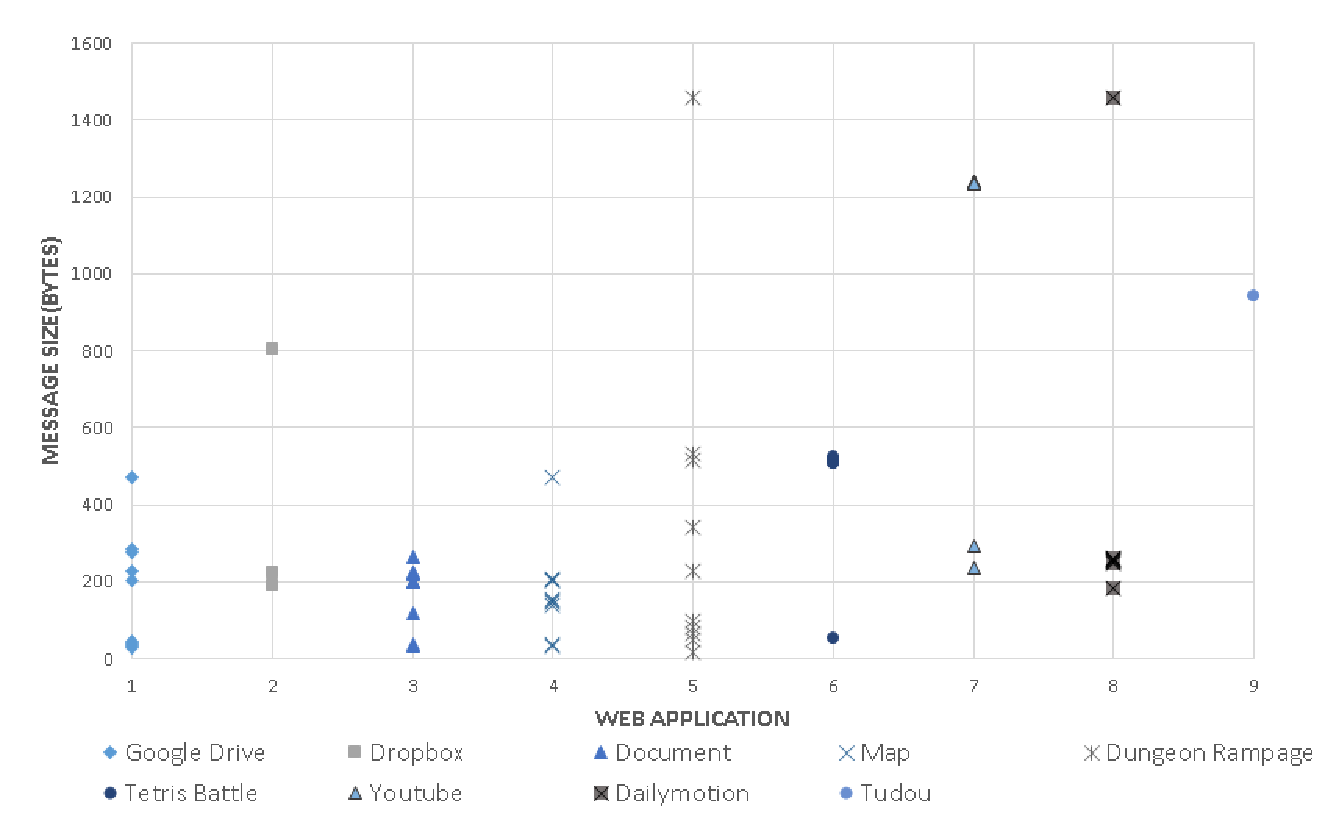
\includegraphics[width=1.0\textwidth]{msg_size_distribution1}
}\\
\subfloat[Firefox]{
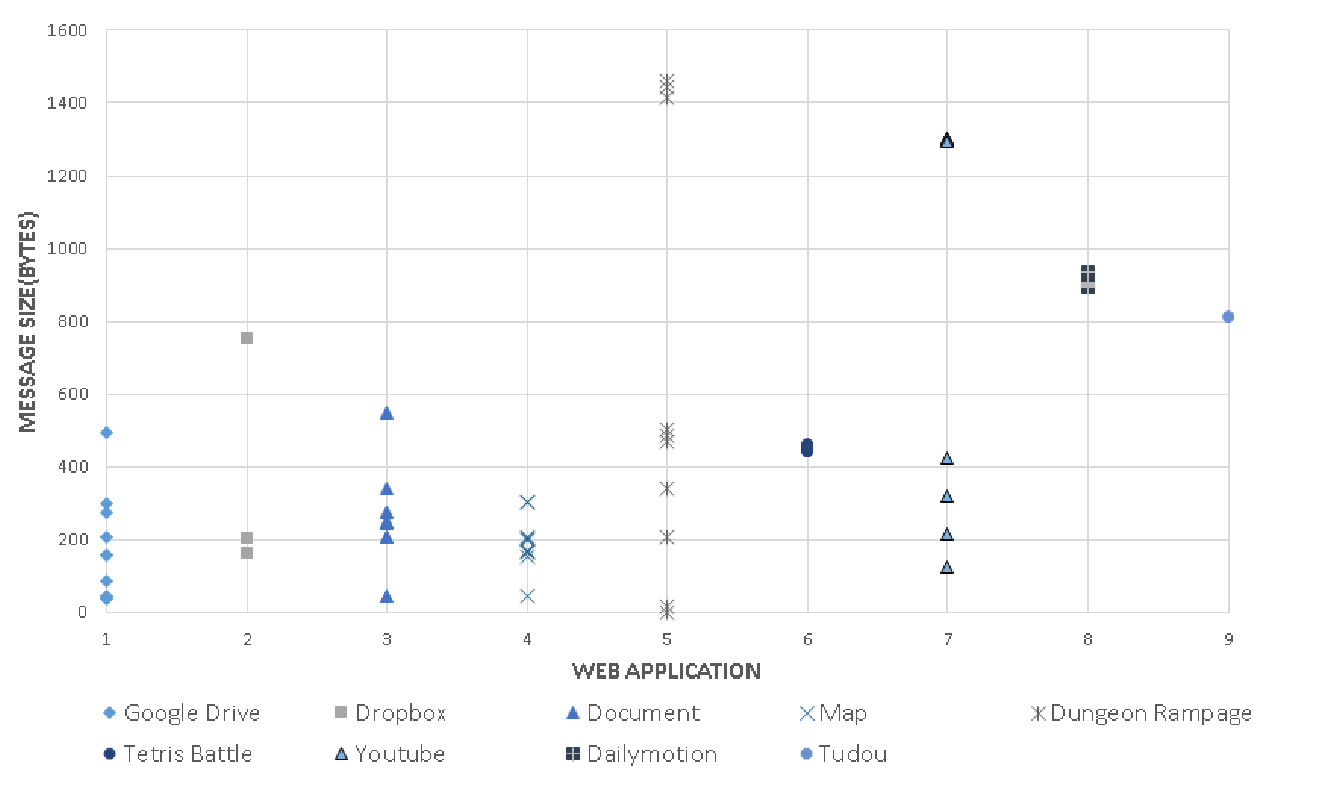
\includegraphics[width=1.0\textwidth]{msg_size_distribution2}
}
\caption{The message size distribution of each web application from two browsers.}
\label{Fig.msg_size_distribution}
\end{figure}

%底下這句的意思是我同樣是在做看影片的動作,但是用不同的平台來觀看會影響feature的結果
Performing the actions on similar web applications will result in different features. For example, the message size distribution of video streaming applications (Youtube, Dailymotion, Tudou) differ obviously according to Figure~\ref{Fig.msg_size_distribution}. However, we do not need to classify individual applications in practice because the management policies (e.g., bandwidth management or QoS) for similar applications are likely to be the same. Thus, we argue that it suffices to classify similar applications into the same category.

Figure~\ref{Fig.setlabel} shows the categorization procedure. We divide the web applications into five categories: file sharing, office, map, game and video streaming. A category consists of one or multiple similar applications. If an application is correctly classified, it is also classified into the correct category. Even though the features are occasionally ambiguous between the applications in the same category (e.g., Dailymotion and Tudou), the applications can be still classified into the category of video streaming applications.   

\begin{figure}[H]
\begin{center} 
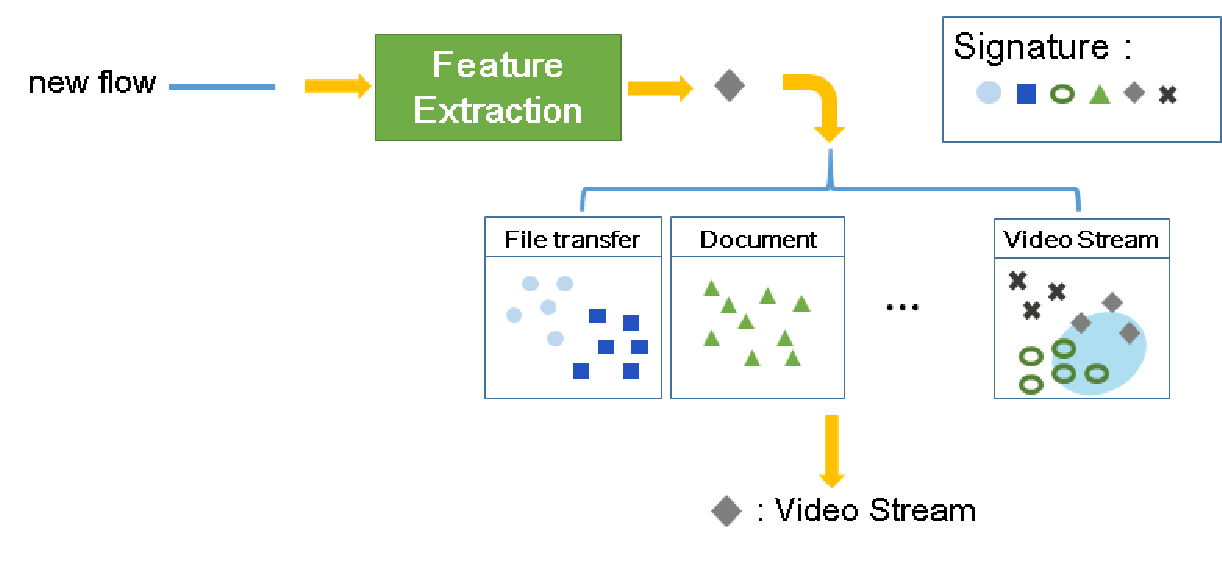
\includegraphics[width=1.0\textwidth]{setlabel}
\end{center}
\caption{Categorization of web applications.}
\label{Fig.setlabel}
\end{figure}


\section{Classification results}
\label{sec:result}
After we collect sufficient data from the browsers, we employ Weka to evaluate whether the feature is effective or not. Weka supports a collection of machine learning algorithms for data mining, among which we choose NBtree, Random Forest, J48graft and Naive Bayes to compare the classification accuracy by using different algorithms. We use 10-fold cross-validation to ensure the reliability. When testing the performance, we divide the web applications into two groups, i.e., interaction applications (document, map, game) and file transfer applications (video streaming, file transfer), since we want to compare the result with the previous method, which tests the accuracy of interaction applications and file transfer applications separately. In addition, the possibility of early classification is also evaluated and it will be described in detail on Section 4.4.4.

We choose the previous study to compare with our mechanism. Lin et al. presented the method based on fine-grained classification and used the average and the standard deviation of the request/response lengths as the features for classification. The difference between our targets is that we only want to classify the kinds of web applications; however, they want to distinguish what action a user does. In the work, they subdivide the flows into search keystrokes, editing, action and download. To dislodge the unnecessary message, they artificially input the first request time or the first request bytes. Nevertheless, that method is more suitable for offline analysis. The reason we choose this study as our comparison is that the way of features extraction ,which is independent of the network condition under the application layer, is similar to our mechanism.

\subsection{Classification with Similar Interactions in Each Run}
Table~\ref{table:inter_accuracy} shows the classification accuracy of each web application. The accuracy of all classifiers reach 95\% or above with our method, but the values still are slightly lower than previous work. There are some reasons may affect the result. For instance, our targets are different and we do not divide search keystroke messages from the flows we extract, since search packets and interaction packets may be transferred in the same connection. The true-positive rate in Google Map does not achieve 1 is because a few instances of Google Map are misidentified as those of Google document.


\begin{table}[H]
\centering
\caption{True/false positive rates of classifying the interactive connections.}
\label{table:inter_accuracy}
\begin{tabular}{|l|l|l|l|l|l|l|l|l|}
\hline
\multirow{2}{*}{} & \multicolumn{2}{l|}{\begin{tabular}[c]{@{}l@{}}Correctly \\ classified\\      (\%)\end{tabular}} 
				  & \multicolumn{2}{l|}{\begin{tabular}[c]{@{}l@{}}Document\\ \\    TP/FP\end{tabular}}                     
				  & \multicolumn{2}{l|}{\begin{tabular}[c]{@{}l@{}}Map \\     \\    TP/FP\end{tabular}}                   
				  & \multicolumn{2}{l|}{\begin{tabular}[c]{@{}l@{}}Game\\ \\              TP/FP\end{tabular}} \\ \cline{2-9} 
                  & Prior & New &Prior & New & Prior & New & Prior & New \\ \hline \hline
NBtree            & 99.80 & 97.50  & \begin{tabular}[c]{@{}l@{}}0.993/\\ 0.001\end{tabular} & \begin{tabular}[c]{@{}l@{}}1/\\ 0.033\end{tabular}   & \begin{tabular}[c]{@{}l@{}}0.999/\\ 0.005\end{tabular}    & 0.90/0  & 1/0    & 1/0  \\ \hline
RandomForest      & 99.89 & 98.75 & \begin{tabular}[c]{@{}l@{}}1/\\ 0.001\end{tabular}     & \begin{tabular}[c]{@{}l@{}}1/\\ 0.017\end{tabular}   & \begin{tabular}[c]{@{}l@{}}0.999/\\ 0\end{tabular}        & 0.95/0 & 1/0    & 1/0  \\ \hline
J48graft          & 99.28 & 97.50  & \begin{tabular}[c]{@{}l@{}}0.993/\\ 0.004\end{tabular} & \begin{tabular}[c]{@{}l@{}}1/\\ 0.033\end{tabular}   & \begin{tabular}[c]{@{}l@{}}0.996/\\ 0.019\end{tabular}    & 0.90/0  & 0.95/0 & 1/0  \\ \hline
NaiveBayes        & 99.49 & 95.00    & \begin{tabular}[c]{@{}l@{}}0.987/\\ 0\end{tabular}     & \begin{tabular}[c]{@{}l@{}}1/\\ 0.067\end{tabular}   & \begin{tabular}[c]{@{}l@{}}0.996/\\ 0.009\end{tabular}    & 0.80/0  & 1/0    & 1/0  \\ \hline
\multicolumn{9}{r}{Prior: Previous work / New : Our method}\\ 

\end{tabular}
\end{table}


%additional web applications
We also chose three additional web applications to disturb classification: Google sheets (type: document), Bing map (type: map) and Dungeon Blitz (type: game). We followed the scenarios described in Table~\ref{table:scenario_app}, and operated each web applications ten times on either Chrome or Firefox. We gathered the features generated from these additional applications and the original training set to verify the accuracy after the disturbance. The result is showed in Table~\ref{table:add_accuracy} and the accuracy after 10-fold cross-validation can be still up to 97.14\% for NBtree. In this work, we add additional applications only to the group of interaction applications to verify the accuracy because the variation of operations for file transfer applications are usually low.


\begin{table}[H]
\centering
\caption{True/false positive rates of classifying the interactive connections with additional web applications.}
\label{table:add_accuracy}
\begin{tabular}{|l|l|l|l|l|l|l|l|l|}
\hline
\multirow{2}{*}{} & \multicolumn{2}{l|}{\begin{tabular}[c]{@{}l@{}}Correctly\\ classified\\ (\%)\end{tabular}} & \multicolumn{2}{l|}{\begin{tabular}[c]{@{}l@{}}Document\\ \\ TP/FP\end{tabular}}                           & \multicolumn{2}{l|}{\begin{tabular}[c]{@{}l@{}}Map\\ \\ TP/FP\end{tabular}} & \multicolumn{2}{l|}{\begin{tabular}[c]{@{}l@{}}Game\\ \\ TP/FP\end{tabular}} \\ \cline{2-9} 
& Orig. & Add. & Orig. & Add. & Orig. & Add. & Orig. & Add.                                                           \\ \hline
NBtree            & 97.50                                       & 97.14                                       & \begin{tabular}[c]{@{}l@{}}1/\\ 0.033\end{tabular} & \begin{tabular}[c]{@{}l@{}}0.975/\\ 0.03\end{tabular} & 0.90/0        & \begin{tabular}[c]{@{}l@{}}0.925/\\ 0.01\end{tabular}       & 1/0          & 1/0                                                           \\ \hline
RandomRorest      & 98.75                                       & 95.71                                       & \begin{tabular}[c]{@{}l@{}}1/\\ 0.017\end{tabular} & \begin{tabular}[c]{@{}l@{}}0.95/\\ 0.04\end{tabular}  & 0.95/0        & \begin{tabular}[c]{@{}l@{}}0.90/\\ 0.02\end{tabular}        & 1/0          & 1/0                                                           \\ \hline
J48graft          & 97.50                                       & 92.14                                       & \begin{tabular}[c]{@{}l@{}}1/\\ 0.033\end{tabular} & \begin{tabular}[c]{@{}l@{}}0.90/\\ 0.06\end{tabular}  & 0.90/0        & \begin{tabular}[c]{@{}l@{}}0.85/\\ 0.04\end{tabular}        & 1/0          & \begin{tabular}[c]{@{}l@{}}0.983/\\ 0.013\end{tabular}        \\ \hline
NaiveBayes        & 95.00                                       & 95.71                                       & \begin{tabular}[c]{@{}l@{}}1/\\ 0.067\end{tabular} & \begin{tabular}[c]{@{}l@{}}0.975/\\ 0.05\end{tabular} & 0.80/0        & \begin{tabular}[c]{@{}l@{}}0.875/\\ 0.01\end{tabular}       & 1/0          & 1/0                                                           \\ \hline
\multicolumn{9}{r}{Orig.: Original training set / Add.: With additional web applications}\\


\end{tabular}
\end{table}


%file transfer applications
We also differentiate between downloading of video stream and general file transfer. We typed a video name and arbitrarily switched to multiple time positions when watching a video or just silently watched a video until the end on Youtube, Dailymotion and Tudou on the two browsers, but we up/downloaded files by Google drive and Dropbox. In summary, we watched 60 videos and transferred 40 files. After extracting the features, we used 10-fold cross-validation to evaluate the classification. It is presented in Table~\ref{table:file_accuracy} that the classification accuracy can be up to 97\% for all the classifiers, even better than previous work. 

\begin{table}[H]
\centering
\caption{True/false positive rates of classifying downloading connections.}
\label{table:file_accuracy}
\begin{tabular}{|l|l|l|l|l|l|l|}
\hline
\multirow{2}{*}{} & \multicolumn{2}{l|}{\begin{tabular}[c]{@{}l@{}}Correctly \\ classified\\ (\%)\end{tabular}} 
                  & \multicolumn{2}{l|}{\begin{tabular}[c]{@{}l@{}}Video\\ Streaming\\ TP/FP\end{tabular}}                    
                  & \multicolumn{2}{l|}{\begin{tabular}[c]{@{}l@{}}Files\\ Transfer\\ TP/FP\end{tabular}}       \\ \cline{2-7} 
& Prior & New & Prior & New & Prior & New  \\ \hline \hline
NBtree            & 92.72                                            & 97.00                                            & \begin{tabular}[c]{@{}l@{}}0.907/\\ 0\end{tabular} & \begin{tabular}[c]{@{}l@{}}0.967/\\ 0.025\end{tabular} & \begin{tabular}[c]{@{}l@{}}1/\\ 0.093\end{tabular} & \begin{tabular}[c]{@{}l@{}}0.975/\\ 0.033\end{tabular} \\ \hline
RandomForest      & 92.33                                            & 97.00                                            & \begin{tabular}[c]{@{}l@{}}0.902/\\ 0\end{tabular} & \begin{tabular}[c]{@{}l@{}}0.967/\\ 0.025\end{tabular} & \begin{tabular}[c]{@{}l@{}}1/\\ 0.098\end{tabular} & \begin{tabular}[c]{@{}l@{}}0.975/\\ 0.033\end{tabular} \\ \hline
J48graft          & 91.57                                            & 97.00                                            & \begin{tabular}[c]{@{}l@{}}0.893/\\ 0\end{tabular} & \begin{tabular}[c]{@{}l@{}}0.967/\\ 0.025\end{tabular} & \begin{tabular}[c]{@{}l@{}}1/\\ 0.107\end{tabular} & \begin{tabular}[c]{@{}l@{}}0.975/\\ 0.033\end{tabular} \\ \hline
NaiveBayes        & 92.72                                            & 97.00                                            & \begin{tabular}[c]{@{}l@{}}0.907/\\ 0\end{tabular} & \begin{tabular}[c]{@{}l@{}}0.967/\\ 0.025\end{tabular} & \begin{tabular}[c]{@{}l@{}}1/\\ 0.093\end{tabular} & \begin{tabular}[c]{@{}l@{}}0.975/\\ 0.033\end{tabular} \\ \hline
\multicolumn{7}{r}{Prior : Previous work / New : Our method}\\ 

\end{tabular}
\end{table}



\subsection{Classification with Diverse Interactions in Each Run}

In this subsection, instead of separating the web applications into interaction function and download function, we classify the traffic into five categories: document, map, game, video stream and file transfer. In the prior study of \cite{TFT14}, the authors evaluated classification separately because the features for interaction function and download function are different in that study, so we also separate the evaluation as well in the last subsection to compare with the prior study fairly. However, we use the same feature, i.e., top-5 most frequent message sizes from the requests, for all the web applications, so we classify all the categories for evaluation in this subsection. We also operated each web application ten times on either Chrome or Firefox, but deliberately performed an extremely different action in the same scenario. For example, we may just continuously type or intermittently edit a document for each time we collected in document function. The classification accuracy after 10-fold cross-validation also can be up to 93.89\% for Random Forest, meaning that the feature is stable and can be used for the classification with high accuracy. 

\begin{table}[H]
\centering
\caption{True/false positive rates of classifying all connections.}
\label{table:all_accuracy}
\begin{tabular}{|l|l|l|l|l|l|l|l|l|l|l|l|l|}
\hline
& \multicolumn{2}{l|}{\begin{tabular}[c]{@{}l@{}}Correctly \\ classified\\  (\%)\end{tabular}} 
& \multicolumn{2}{l|}{\begin{tabular}[c]{@{}l@{}}Document\\ \\ TP/FP\end{tabular}} 
& \multicolumn{2}{l|}{\begin{tabular}[c]{@{}l@{}}Map\\ \\ TP/FP\end{tabular}} 
& \multicolumn{2}{l|}{\begin{tabular}[c]{@{}l@{}}Game\\ \\ TP/FP\end{tabular}} 
& \multicolumn{2}{l|}{\begin{tabular}[c]{@{}l@{}}Video\\  Streaming\\    TP/FP\end{tabular}} 
& \multicolumn{2}{l|}{\begin{tabular}[c]{@{}l@{}}Files\\ Transfer\\ TP/FP\end{tabular}} \\ \hline \hline
NBtree       & \multicolumn{2}{l|}{92.22}                                                                       & \multicolumn{2}{l|}{\begin{tabular}[c]{@{}l@{}}1/\\ 0.05\end{tabular}}                 & \multicolumn{2}{l|}{\begin{tabular}[c]{@{}l@{}}0.80/\\ 0.006\end{tabular}}         & \multicolumn{2}{l|}{\begin{tabular}[c]{@{}l@{}}0.95/\\ 0.007\end{tabular}}   & \multicolumn{2}{l|}{\begin{tabular}[c]{@{}l@{}}0.917/\\ 0\end{tabular}}                  & \multicolumn{2}{l|}{\begin{tabular}[c]{@{}l@{}}0.925/\\ 0.029\end{tabular}}           \\ \hline
RandomForest & \multicolumn{2}{l|}{93.89}                                                                       & \multicolumn{2}{l|}{\begin{tabular}[c]{@{}l@{}}0.90/\\ 0.013\end{tabular}}              & \multicolumn{2}{l|}{\begin{tabular}[c]{@{}l@{}}0.90/\\ 0.019\end{tabular}}         & \multicolumn{2}{l|}{\begin{tabular}[c]{@{}l@{}}0.975/\\ 0.021\end{tabular}}  & \multicolumn{2}{l|}{\begin{tabular}[c]{@{}l@{}}0.933/\\ 0.017\end{tabular}}              & \multicolumn{2}{l|}{\begin{tabular}[c]{@{}l@{}}0.95/\\ 0.007\end{tabular}}            \\ \hline
J48graft     & \multicolumn{2}{l|}{92.22}                                                                       & \multicolumn{2}{l|}{\begin{tabular}[c]{@{}l@{}}0.95/\\ 0.031\end{tabular}}             & \multicolumn{2}{l|}{\begin{tabular}[c]{@{}l@{}}0.80/\\ 0.013\end{tabular}}         & \multicolumn{2}{l|}{\begin{tabular}[c]{@{}l@{}}0.975/\\ 0.021\end{tabular}}  & \multicolumn{2}{l|}{\begin{tabular}[c]{@{}l@{}}0.917/\\ 0.008\end{tabular}}              & \multicolumn{2}{l|}{\begin{tabular}[c]{@{}l@{}}0.925/\\ 0.021\end{tabular}}           \\ \hline
NaiveBayes   & \multicolumn{2}{l|}{92.22}                                                                       & \multicolumn{2}{l|}{\begin{tabular}[c]{@{}l@{}}0.95/\\ 0.025\end{tabular}}             & \multicolumn{2}{l|}{\begin{tabular}[c]{@{}l@{}}0.95/\\ 0.013\end{tabular}}        & \multicolumn{2}{l|}{\begin{tabular}[c]{@{}l@{}}0.95/\\ 0.029\end{tabular}}   & \multicolumn{2}{l|}{\begin{tabular}[c]{@{}l@{}}0.917/\\ 0.017\end{tabular}}              & \multicolumn{2}{l|}{\begin{tabular}[c]{@{}l@{}}0.875/\\ 0.014\end{tabular}}           \\ \hline
\end{tabular}
\end{table}

\subsection{Classification with Interactions from Multiple Users}

To ensure the accuracy does not too depend on specific users, we invited eight users to generate the traffic for the classification. In this subsection, we compare only interactive functions because the their actions are more diverse than download functions. The users were asked to perform similar actions to those from a single user and repeated three times for each web applications on Chrome and Firefox. The total number of packet traces is 192: 48 for Google document, 48 for Google map, 48 for Dungeon Rampage and 48 for Tetris Battle.

Table~\ref{table:multi_accuracy} shows the accuracy for each algorithm. We also used 10-fold cross-validation for this classification. The accuracy of our method for Naive Bayes is even higher than the results in Section 4.4, and can be up to 97.92\% with random forest. Compared the result with the training set shown in last subsection, the accuracy is degraded just slightly, meaning that the feature is stable. 

\begin{table}[H]
\centering
\caption{True/false positive rates of classifying the interactive connections for multiple users.}
\label{table:multi_accuracy}
\begin{tabular}{|l|l|l|l|l|l|l|l|l|}
\hline
\multirow{2}{*}{} & \multicolumn{2}{l|}{\begin{tabular}[c]{@{}l@{}}Correctly \\ classified\\      (\%)\end{tabular}} 
				  & \multicolumn{2}{l|}{\begin{tabular}[c]{@{}l@{}}Document\\ \\    TP/FP\end{tabular}}                     
				  & \multicolumn{2}{l|}{\begin{tabular}[c]{@{}l@{}}Map \\     \\    TP/FP\end{tabular}}                   
				  & \multicolumn{2}{l|}{\begin{tabular}[c]{@{}l@{}}Game\\ \\              TP/FP\end{tabular}} \\ \cline{2-9} 
                  & Prior & New & Prior & New & Prior & New & Prior & New \\ \hline \hline

NBtree            & 96.63                                        & 96.35                                        & \begin{tabular}[c]{@{}l@{}}0.939/\\ 0.025\end{tabular} & \begin{tabular}[c]{@{}l@{}}0.938/\\ 0.028\end{tabular} & \begin{tabular}[c]{@{}l@{}}0.971/\\ 0.044\end{tabular} & \begin{tabular}[c]{@{}l@{}}0.938/\\ 0.021\end{tabular} & \begin{tabular}[c]{@{}l@{}}0.993/\\ 0\end{tabular}     & 0.99/0                                                 \\ \hline
RandomForest     & 98.28                                        & 97.92                                        & \begin{tabular}[c]{@{}l@{}}0.954/\\ 0.009\end{tabular} & \begin{tabular}[c]{@{}l@{}}1/\\ 0.007\end{tabular}     & \begin{tabular}[c]{@{}l@{}}0.99/\\ 0.032\end{tabular}  & \begin{tabular}[c]{@{}l@{}}0.979/\\ 0.014\end{tabular} & 1/0                                                    & \begin{tabular}[c]{@{}l@{}}0.969/\\ 0.01\end{tabular}  \\ \hline
J48graft         & 97.65                                        & 93.75                                        & \begin{tabular}[c]{@{}l@{}}0.939/\\ 0.011\end{tabular} & \begin{tabular}[c]{@{}l@{}}0.917/\\ 0.035\end{tabular} & \begin{tabular}[c]{@{}l@{}}0.986/\\ 0.044\end{tabular} & \begin{tabular}[c]{@{}l@{}}0.917/\\ 0.035\end{tabular} & \begin{tabular}[c]{@{}l@{}}0.993/\\ 0.001\end{tabular} & \begin{tabular}[c]{@{}l@{}}0.958/\\ 0.021\end{tabular} \\ \hline
NaiveBayes       & 95.74                                        & 95.83                                        & \begin{tabular}[c]{@{}l@{}}0.87/\\ 0.017\end{tabular}  & \begin{tabular}[c]{@{}l@{}}0.938/\\ 0.028\end{tabular} & \begin{tabular}[c]{@{}l@{}}0.98/\\ 0.091\end{tabular}  & \begin{tabular}[c]{@{}l@{}}0.938/\\ 0.028\end{tabular} & \begin{tabular}[c]{@{}l@{}}1/\\ 0.001\end{tabular}     & \begin{tabular}[c]{@{}l@{}}0.979/\\ 0\end{tabular}     \\ \hline

\multicolumn{9}{r}{Pre: Previous work / New : Our method}\\ 

\end{tabular}
\end{table}


\subsection{Early Classification}
\label{sec:early}
The classification method in this work can be applied to manage various web applications, even though the web traffic is encrypted. The specifics of classification may vary in practice, depending on the purpose of management. If the purpose is accounting the usage of web applications in a network, it would suffice to classify the web applications offline based on the features from \emph{the entire packet traces} that have been observed. However, if the purpose is access control, classification after extracting the features from the entire packet traces will be too late to block the traffic in time. Thus, we also evaluate the effectiveness of early classification with the features from the partial messages in the beginning of the connections. In early classification, a connection can be blocked as soon as the web application is recognized based on the features from the partial messages. 

The packet traces for evaluating early classification are same as those described in the last subsection. We extracted the first $k$ messages from each main connection ($k=15, 20, 25, 30, 50, 100$) and used the size distribution of only these messages for the evaluation. Like the features from the entire packet traces, we also extracted the top five frequent message sizes in terms of occurrence frequency.  

The previous analysis show that the true-positive rate of almost all kinds of functions are at least up to 0.90; however, the true-positive rate for the map application is decreased to 0.80 because its features are not so stable as others. We choose Dungeon Rampage on Chrome as example for stable one shown as Figure~\ref{Fig.set_size_dr} and Google map on Chrome as example for unstable one shown as Figure~\ref{Fig.set_size_map}. The line chart is created by entire messages within a main connection and the scatter chart is created by the first $k$ messages in each figure.

\begin{figure}[H]
\begin{center} 
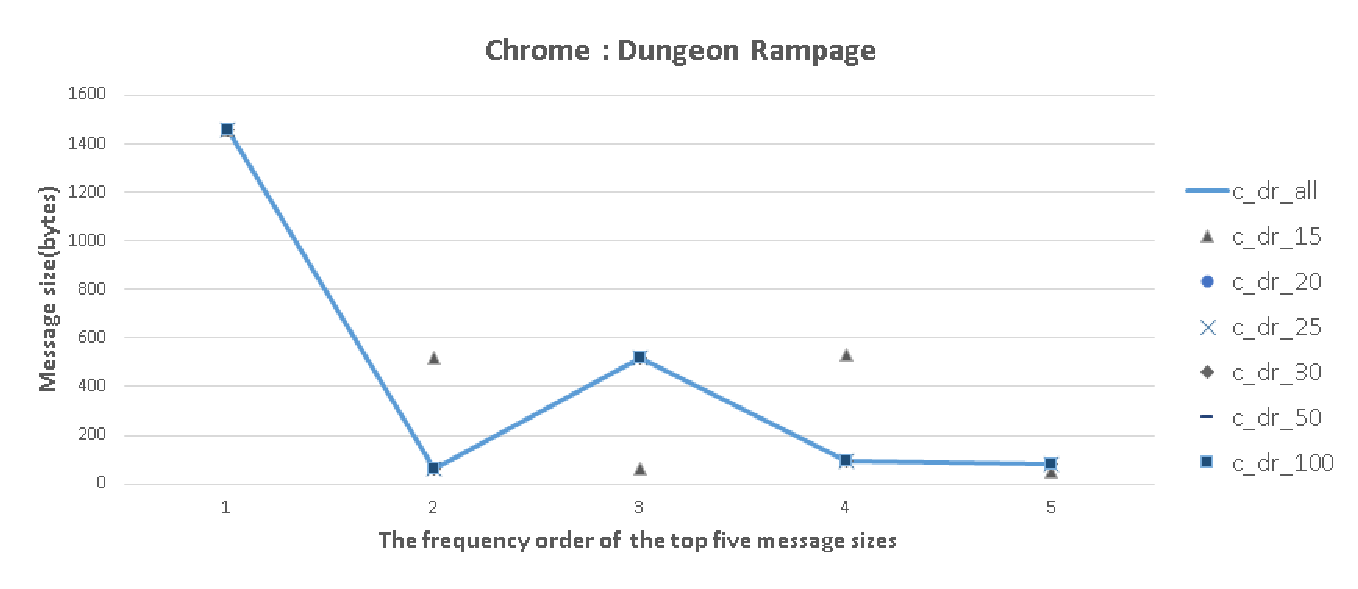
\includegraphics[width=1.1\textwidth]{early_dr}
\end{center}
\caption{The message size distribution for Dungeon Rampage.}
\label{Fig.set_size_dr}
\end{figure}

Figure~\ref{Fig.set_size_dr} depicts that the scatter charts are similar with the trend of line chart when we extract more than the first 20 messages. Figure~\ref{Fig.set_size_map} depicts that the scatter charts are almost similar with the trend of line chart when we extract more than the first 30 messages. So we finally extracted the first 30 messages from each web applications as our feature for early classification. The classification accuracy after 10-fold cross-validation can be at least 86.67\% and even can be up to 93.89\% for Random Forest.


\begin{figure}[H]
\begin{center} 
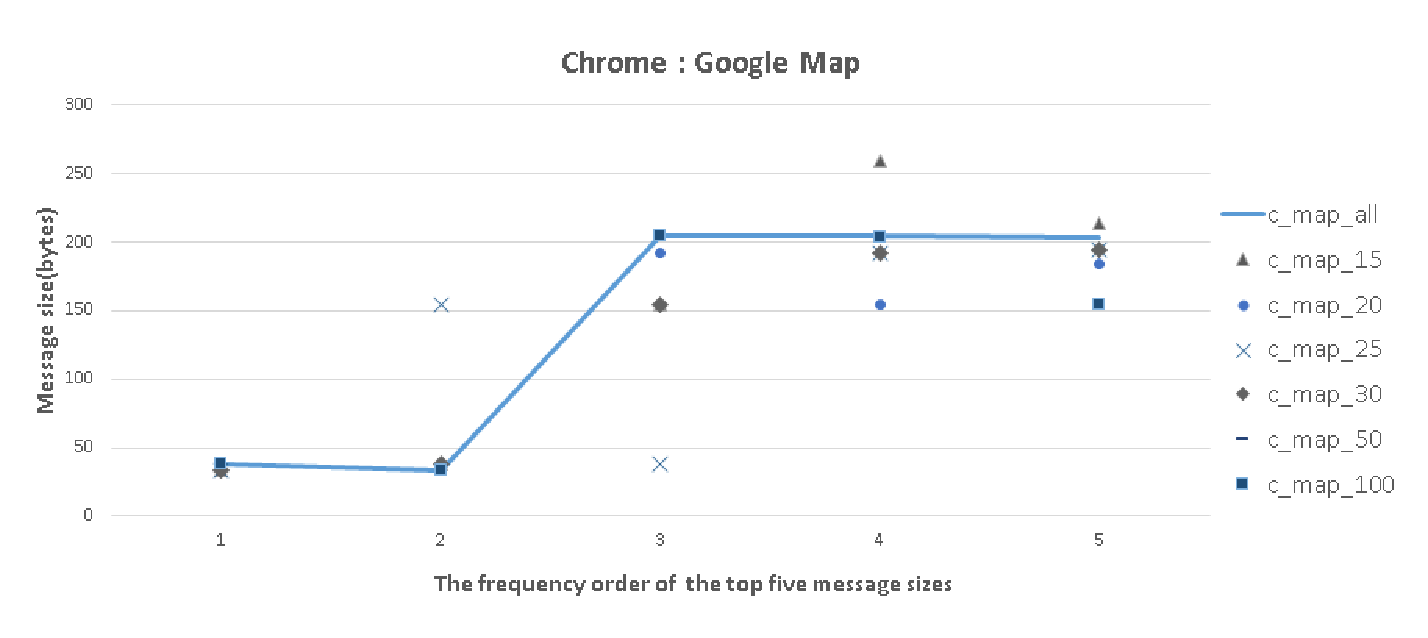
\includegraphics[width=1.1\textwidth]{early_map}
\end{center}
\caption{The message size distribution for Google map.}
\label{Fig.set_size_map}
\end{figure}

\begin{table}[H]
\centering
\caption{Early classification true/false positive rate in all connections.}
\label{table:early_accuracy}
\begin{tabular}{|l|l|l|l|l|l|l|}
\hline
& \begin{tabular}[c]{@{}l@{}}Correctly \\ classified\\ (\%)\end{tabular} 
& \begin{tabular}[c]{@{}l@{}}Document\\ \\ TP/FP\end{tabular} 
& \begin{tabular}[c]{@{}l@{}}Map \\ \\ TP/FP\end{tabular} 
& \begin{tabular}[c]{@{}l@{}}Game\\ \\ TP/FP\end{tabular} 
& \begin{tabular}[c]{@{}l@{}}Video\\ Stream\\ TP/FP\end{tabular} 
& \begin{tabular}[c]{@{}l@{}}File\\ Transfer\\ TP/FP\end{tabular} \\ \hline \hline
NBtree       & 86.67         & \begin{tabular}[c]{@{}l@{}}0.70/\\ 0.038\end{tabular}  & \begin{tabular}[c]{@{}l@{}}0.95/\\ 0.019\end{tabular}         & \begin{tabular}[c]{@{}l@{}}0.925/\\ 0.007\end{tabular}           & \begin{tabular}[c]{@{}l@{}}0.933/\\ 0.025\end{tabular} & \begin{tabular}[c]{@{}l@{}}0.75/\\ 0.079\end{tabular}           \\ \hline
RandomForest & 93.89         & \begin{tabular}[c]{@{}l@{}}0.85/\\ 0.013\end{tabular}  & 1/0                                                           & \begin{tabular}[c]{@{}l@{}}1/\\ 0.014\end{tabular}           & \begin{tabular}[c]{@{}l@{}}0.933/\\ 0.017\end{tabular} & \begin{tabular}[c]{@{}l@{}}0.90/\\ 0.036\end{tabular}           \\ \hline
J48graft     & 88.33         & \begin{tabular}[c]{@{}l@{}}0.85/\\ 0.019\end{tabular}  & \begin{tabular}[c]{@{}l@{}}1/\\ 0.019\end{tabular}            & \begin{tabular}[c]{@{}l@{}}0.95/\\ 0.029\end{tabular}           & \begin{tabular}[c]{@{}l@{}}0.85/\\ 0.042\end{tabular}  & \begin{tabular}[c]{@{}l@{}}0.825/\\ 0.043\end{tabular}          \\ \hline
NaïveBayes   & 87.22         & \begin{tabular}[c]{@{}l@{}}0.85/\\ 0.063\end{tabular}  & \begin{tabular}[c]{@{}l@{}}0.95\\ /0.013\end{tabular}         & \begin{tabular}[c]{@{}l@{}}0.925/\\ 0.021\end{tabular}           & \begin{tabular}[c]{@{}l@{}}0.95/\\ 0.017\end{tabular}  & \begin{tabular}[c]{@{}l@{}}0.675/\\ 0.043\end{tabular}          \\ \hline
\end{tabular}
\end{table}

\section{Practice and Limitation}
\label{sec:app_limit}

Even though the classification accuracy is high for extracted packet traces from real user interactions with web applications, there are still some issues that should be addressed to deploy this classification in practice.

First, although one IP address may be associated with more than one web application, as we demonstrated earlier in this work, we can still record the mapping between the IP addresses and their associated applications from earlier classification in a list to speed up classification. Since the mapping may be one-to-many, if a remote IP address can be found in the list and it is mapped to only one application, we can leverage the result of earlier classification to label the traffic to that application directly; otherwise, we can follow the procedure described in Chapter 3 to classify the web application. The result from earlier classification can at least help reduce the scope of possible labels.

Second, the traffic for each packet trace is just generated from a specific web application in this work, but in reality, we will need to analyze multiple applications at the same time and extracting the main connection is a problem. To solve this issue, we will observe the traffic density and quantity of each IP address during a period time and if the values both reach the thresholds, we will extract it as the main connection for classification. After classification, if the device that employs the design determines to block the main connection, the connections having the same pair of source/destination IP addresses as the main connection and happening around it will be blocked as well. Furthermore, users may use a web application not in the training set. Thus, after traffic classification, we will have to compute the distance between the feature vectors of the analyzed traffic and the application(s) that the analyzed traffic is supposed to be. If the distance is too long, than the analyzed traffic will be labeled as unknown.


Third, if the main connection is identified after the web application has been executed for a period of time, it may be too late to block an application for access control since the function is likely to have already completed its execution when the flows are collected and analyzed. The early classification described in Section~\ref{sec:early} can address this issue. Moreover, the accuracy may be decreased if the execution time of an web application function is too short to extract meaningful feature. 

\chapter{Conclusion and future work}
\label{conclusion}
In this work, we discuss the hazard that an compromised switch in SDN network may bring. In the scenario we set up, we can see how the problems can be solved by using SDN features. Even a different scenario is met, we believe that the new problems it introduces can also be solved with some extension and adjustment with the functionality SDN provides. We propose an effective way that is able to scan through the entire network for disobedient forwarding behavior with less number of packets, and evaluate it under different network topology types, scales and entry numbers on each switch. The experimental result demonstrates that our method is effective under a network topology with balance structure. Also, the scale of the network topology does not affect the efficiency significantly, and the aggregation rate grows to 3.48 in fat tree topology once there are 120 entries in each switch. 

We can only anticipate what the attackers may try to target with SDNs. The deployments are new, the protocols are new, the controller software is new, and the history of past SDN attacks is unknown. Based on the SDN architecture, we can predict where an attacker may be likely to strike. If we put ourselves in the attacker\textquotesingle s shoes, we might be able to spot a weakness to exploit. Then we can harden that weakness ahead of time. Before an organization embarks on an SDN deployment project, they should consider how they would secure the system during the early design stage. 

In the future work, more realistic factors should be taken into consideration, such as the collaboration of multiple compromised switches and the entries with multiple match fields and wildcard fields. Furthermore, the aggregated group finding method currently performs DFS without any estimation, the core algorithm can be improved by adding heuristic function. Also, as the new versions of OpenFlow are released, the method should be able to be optimized with the support of the new features. For example, the auxiliary entries can be installed on the egress table once it is fully supported.


\begin{thebibliography}{1}

\bibitem{KRVRAU15} %journal
D. Kreutz, F. M. Ramos, P.E. Verissimo, C.E. Rothenberg, S. Azodolmolky and S. Uhlig,
``Software-Defined Networking: A Comprehensive Survey,'' In Proceeedings of the IEEE, vol. 103, no. 1, pp.  14-76, Jan. 2015.

\bibitem{MABPPRST08}
N. McKeown, T. Anderson, H. Balakrishnan, G. Parulkar, L. Peterson, J. Rexford, S. Shenker and J. Turner,
``OpenFlow: Enabling Innovation in Campus Networks,'' ACM SIGCOMM Computer Communication Review, vol. 38, issue 2, pp. 69-74, Apr. 2008.

\bibitem{LHM10} %conf
B. Lantz, B. Heller and N. McKeown,
``A Network in a Laptop: Rapid Prototyping for Software-Defined Network,'' In Proc. of the 9th ACM SIGCOMM Workshop on Hot Topics in Networks, Oct. 2010.

\bibitem{OF_SPEC}
OpenFlow Switch Version 1.5 Specification, \url{https://www.opennetworking.org/images/stories/downloads/sdn-resources/onfspecifications/openflow/openflow-switch-v1.5.1.pdf}.

\bibitem{SOS13}
S. Scott-Hayward, G. O’Callaghan and S. Sezer,
``SDN Security: A Survey,'' In Proc. of IEEE SDN for Future Networks and Services (SDN4FNS), pp. 1–7., Nov. 2013.

\bibitem{CM}
M. Coughlin,
``A Survey of SDN Security Research,'' \url{http://ngn.cs.colorado.edu/~coughlin/doc/a_survey_of_sdn_security_research.pdf}.

\bibitem{HXWG15}
S. Hong, L. Xu, H. Wang and G. Gu,
``Poisoning Network Visibility in Software-Defined Networks: New Attacks and Countermeasures,''  In Proceedings of the 22th Annual Network and Distributed System Security Symposium (NDSS), Feb. 2015.

\bibitem{CKGL15}
P. W. Chi, C. T. Kuo, J. W. Guo and C. L. Lei,
``How to Detect a Compromised SDN Switch,'' In Proc. of the 1st IEEE Conference Network of Softwarization (NetSoft), pp. 1-6., Apr. 2015.

\bibitem{PJL16}
C. Pang, Y. Jiang and Q. Li,
``FADE: Detecting Forwarding Anomaly in Software-Defined Networks,'' In Proc. IEEE International Conference of Communications (ICC), May 2016.

\bibitem{ZKVM12}
H. Zengyz, P. Kazemianyz, G. Varghese and N. McKeowny,
``Automatic Test Packet Generation,'' In Proc. of the 8th International Conference on Emerging Networking Experiments and Technologies (CoNEXT), Dec. 2012.

\bibitem{HP_SPEC}
HP OpenFlow 1.3 Administrator Guide, \url{http://h10032.www1.hp.com/ctg/Manual/c04495114}.

\bibitem{OVS_OFCTL}
OpenvSwitch Manual, \url{http://openvswitch.org/support/dist-docs/ovs-ofctl.8.txt}.

\bibitem{LAB14}
L. Schehlmann, A. Sebastian and B. Harald, 
``Blessing or curse? Revisiting security aspects of Software-Defined Networking,'' In Proc. of 10th IEEE International Conference on Network and Service Management (CNSM), Nov. 2014.

\bibitem{KJK}
A. Khandelwal, N. Jain and S. Kamara,
``Attacking Data Center Networks from the Inside,'' \url{https://www.microsoft.com/en-us/research/wp-content/uploads/2016/02/dcn.pdf}.

\bibitem{TTB15}
T. THANH BUI,
``Analysis of Topology Poisoning Attacks in Software-Defined Networking,'' Degree project in security and mobile computing, Second Level Stockholm, Aug. 2015.

\bibitem{ATPP15}
T. Alharbi, M. Portmann and F. Pakzad,
``The (In) Security of Topology Discovery in Software Defined Networks,'' In Proc. of 40th IEEE Conference on Local Computer Networks (LCN), Oct. 2015.
 
\bibitem{AAS14}
M. Antikainen, T. Aura and M. Särelä,
``Spook in Your Network: Attacking an SDN with a Compromised OpenFlow Switch,'' In Proc. of Nordic Conference on Secure IT System (NordSec), Oct. 2014.

\bibitem{ARDC14}
K. Agarwal, E. Rozner, C. Dixon and J. Carter,
``SDN traceroute: Tracing SDN Forwarding without Changing Network Behavior,'' In Proc. of the 3rd ACM Workshop on HotTopics in Software Defined Networking (HotSDN), Aug. 2014.

\bibitem{BCKK15}
R. Bifulco, H. Cui, G. O. Karame and F. Klaedtke,
``Fingerprinting software-defined networks,'' In Proc. of 2015 IEEE 23rd International Conference on Network Protocols (ICNP), Nov. 2015.

\bibitem{DMR97}
D. Karger, M. Rajeev and G. D. S. Ramkumar,
``On approximating the longest path in a graph,'' in Algorithmica, pp. 82-98, May 1997.

\bibitem{RU04}
R. Uehara and Y. Uno,
``Efficient algorithms for the longest path problem,'' in Algorithms and Computation, Springer Berlin Heidelberg, pp. 871-883, Dec. 2005.


\bibitem{Mininet}
Mininet Official Website, \url{http://mininet.org/}.

\bibitem{FNSS}
Topology Package In FNSS API Documentation, \url{http://fnss.github.io/doc/core/apidoc/fnss.functions.html#topologies-package}.

\bibitem{PACKETOUT}
Flowgrammable SDN OpenFlow Doumentation Message-Layer Section, \url{http://flowgrammable.org/sdn/openflow/message-layer/packetout/}.

\bibitem{MPFHMRSV09}
R. Niranjan Mysore, A. Pamboris, N. Farrington, N. Huang, P. Miri, S. Radhakrishnan, V. Subramanya and A. Vahdat, ``PortLand: A Scalable Fault-Tolerant Layer 2 Data Center Network Fabric,'' ACM SIGCOMM Computer Communication Review, Vol. 39, no. 4, pp. 39-50., Aug. 2009.

\bibitem{PORT_FREQ}
Network Traffic Breakdown By Protocol Discussion On WhatPulse, \url{http://dkqnkzjkqr9h2.cloudfront.net/forums/showthread.php?tid=6987}.
\end{thebibliography}
\end{document}